\documentclass[aspectratio=169]{beamer}
\usepackage{adjustbox}
\usepackage[utf8]{inputenc}
\usepackage{tikz}
\usepackage{hyperref}
\usepackage{multimedia}
\usepackage{ulem}
\usepackage{wasysym}
\usetikzlibrary{mindmap,trees}

\usepackage{pbox}

\usepackage[absolute,overlay]{textpos}

% \usetikzlibrary{mindmap,trees}

\usepackage{smartdiagram}
\usetikzlibrary{shapes.geometric,calc}
\usetikzlibrary{shapes.symbols}
\usetikzlibrary{shapes.symbols,positioning}
\usepackage{metalogo}

\usetikzlibrary{backgrounds, calc, shadows, shadows.blur}

\newcommand\addcurlyshadow[2][]{
    % #1: Optional aditional tikz options
    % #2: Name of the node to "decorate"
    \begin{pgfonlayer}{background}
        \path[blur shadow={shadow xshift=0pt, shadow yshift=0pt, shadow blur steps=6}, #1]
        ($(#2.north west)+(.3ex,-.5ex)$)
        -- ($(#2.south west)+(.5ex,-.7ex)$)
        .. controls ($(#2.south)!.3!(#2.south west)$) .. (#2.south)
        .. controls ($(#2.south)!.3!(#2.south east)$) .. ($(#2.south east)+(-.5ex,-.7ex)$)
        -- ($(#2.north east)+(-.3ex, -.5ex)$)
        -- cycle;
   \end{pgfonlayer}
}


%%%%%%%%%%%%%%%%%%%%%%%%%%%%%%%%%%%%%%%%%%%%%%%%%%%%%%%%%%%%%%%%%%%
% Style modifications
%%%%%%%%%%%%%%%%%%%%%%%%%%%%%%%%%%%%%%%%%%%%%%%%%%%%%%%%%%%%%%%%%%%

\usetheme{Berlin}

%%% Fonts %%%

% Change font. Fontspec requires xelatex instead of pdflatex!
% Font catalog: https://www.tug.dk/FontCatalogue/
\usepackage{fontspec}

%\setsansfont{Comfortaa}
%\setsansfont{DejaVu Sans}
%\setsansfont{Fira Sans}

% Use "Fira Sans Light" as the normal font and the "Fira Sans" for
% bold fonts

\setsansfont[
  ItalicFont={Fira Sans Light Italic},
  BoldFont={Fira Sans},
  BoldItalicFont={Fira Sans Italic}]{Fira Sans Light}

\setbeamerfont{title}{size=\Large, series=\bfseries}
\setbeamerfont{frametitle}{size=\large, series=\bfseries}

%%% Slide template %%%

\setbeamertemplate{frames}[default]

% Empty headline / footline
\setbeamertemplate{headline}{}
\setbeamertemplate{footline}{}

% Remove navigation icons
\setbeamertemplate{navigation symbols}{}

%%% Colors %%%

\usecolortheme{crane}

\definecolor{lightgray}{RGB}{220,220,220}
\definecolor{darkgray}{RGB}{45,45,45}
%\definecolor{darkblue}{RGB}{0,86,137}
\definecolor{darkblue}{RGB}{22,90,151} % Blue of the Gießen Website
\definecolor{lightblue}{RGB}{229, 245, 255}

\definecolor{darkblue}{RGB}{208,29,44}


% Use the slide background in block environments                                                                                                      
\setbeamercolor{title}{fg=white,bg=darkblue}
\setbeamertemplate{blocks}[default]
\setbeamercolor{block title}{bg=}
\setbeamercolor{block body}{bg=lightgray}
\setbeamercolor{frametitle}{fg=white,bg=darkblue}
\setbeamerfont{block body}{size=\large}
\setbeamercolor{itemize item}{fg=black}
\setbeamertemplate{itemize items}[circle]
\setbeamercolor{section number projected}{bg=darkblue,fg=white}
\setbeamercolor{section in toc}{fg=black}
\setbeamercolor{subsection in toc}{fg=darkblue}

\addtobeamertemplate{block begin}{\pgfsetfillopacity{0.8}}{\pgfsetfillopacity{1}}
\addtobeamertemplate{frametitle}{\pgfsetfillopacity{1.0}}{\pgfsetfillopacity{1}}
\addtobeamertemplate{title page}{\pgfsetfillopacity{1.0}}{\pgfsetfillopacity{1}}

% Command to place the test (e.g. citation) in the center of the footer
\newcommand{\setfootercentertext}[1]{
  \setbeamertemplate{footline}{
    \hspace*{\fill}
    \raisebox{3mm}[0mm][0mm]{
      \tiny{#1}}\hspace*{\fill}}
}

%%%%%%%%%%%%%%%%%%%%%%%%%%%%%%%%%%%%%%%%%%%%%%%%%%%%%%%%%%%%%%%%%%%
% Content
%%%%%%%%%%%%%%%%%%%%%%%%%%%%%%%%%%%%%%%%%%%%%%%%%%%%%%%%%%%%%%%%%%%

%------------------------------------------------------------------------------
\title{Supervised Machine Learning Methods}
%------------------------------------------------------------------------------

\author{\small Konrad U. Förstner}

\institute{ZB MED -- Information Centre for Life Science \& TH Köln}

\date{\scriptsize 
  Workshop \textit{Systems Biology: From large datasets to biological insight}\\
  at the European Bioinformatics Institute\\
  2019-07-10\\\ \\
  % \includegraphics[width=1.0cm]{images/vcard_qr_code.png}\ \\ \ \\
  %
\includegraphics[width=0.88cm]{images/creative_commons_attribute.png}
}

\logo{
  
\includegraphics[height=1.0cm]{images/ZBMED_2017_EN.pdf}
  
\includegraphics[height=0.8cm]{images/logo_TH-Koeln_CMYK_22pt.eps}
}

\begin{document}

%\setbeamertemplate{background}{
  % \includegraphics[height=\paperheight]{images/flickr_normanbleventhalmapcenter_2710796662_mod.jpg}
%}

\begin{frame}{}
  \titlepage
\end{frame}
\logo{}

\begin{frame}{}
  \frametitle{Small survey before we start}

  \begin{block}{}
    \begin{center}    
      Who is already familiar with ...
      \begin{itemize}
      \item ... supervised machine learning -
        classification and regression?
      \item ... Python?
      \item ... Jupyter Notebooks?
      \item ... scikit-learn?
      \end{itemize}
    \end{center}
  \end{block}

\end{frame}

\setcounter{tocdepth}{1}
\begin{frame}{}
   \tableofcontents
\end{frame}

%%%%%%%%%%%%%%%%%%%%%%
\section{Introduction}
%%%%%%%%%%%%%%%%%%%%%%

\begin{frame}{}
   \tableofcontents[currentsection]
\end{frame}

\begin{frame}

  \begin{center}
    \begin{adjustbox}{max totalsize={.9\textwidth}{.7\textheight},center}
    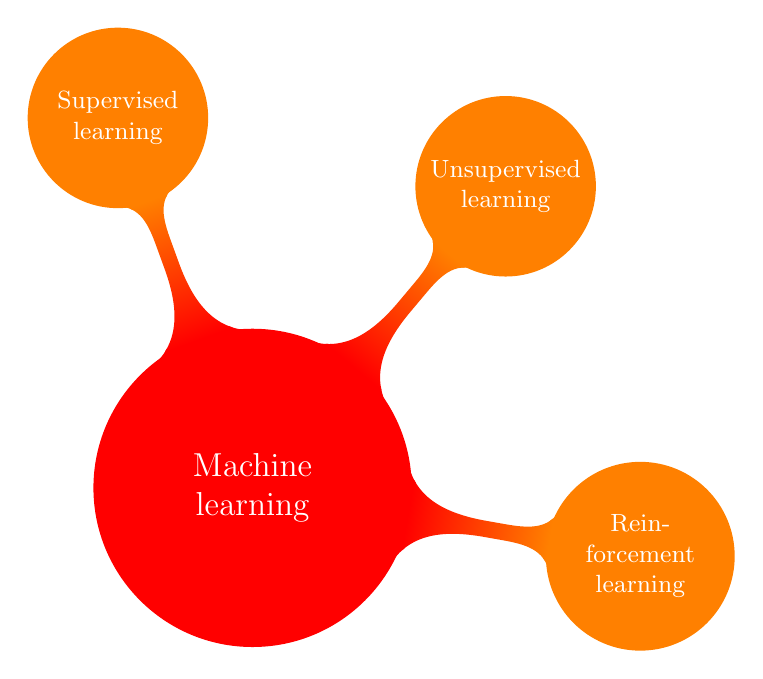
\begin{tikzpicture}
      \path[mindmap,concept color=red,text=white]
      node[concept] {Machine\\learning}
      [clockwise from=110]
      
      child[concept color=orange] { node[concept] {Supervised learning}}
      child[concept color=orange] { node[concept] {Unsuper\-vised learning}}
      child[concept color=orange] { node[concept] {Rein\-forcement learning}}

      ;
    \end{tikzpicture}  
    \end{adjustbox}
  \end{center}
  
\end{frame}

\begin{frame}
  \frametitle{Basic concept of supervised machine learning}

  \begin{block}{}
      \begin{center}
      Supervised learning means to generalize from given examples.\\
      \ \\
      Mapping from input X (two-dimensional matrix) to output vectore y\\
      (label for classification, values for regression).\\
      \ \\
      
      $X_{1} \rightarrow y_{1}$\\
      $X_{2} \rightarrow y_{2}$\\
      $X_{3} \rightarrow y_{3}$\\

      \ \\
      Generating a function to map input variables ($X$) to an output
      variable $y$. \\
      \ \\
      $y = f(X)$
      \end{center}
    \end{block}
\end{frame}

\begin{frame}
  \frametitle{Two tasks that can be solved with supervised learning}
  \begin{center}
    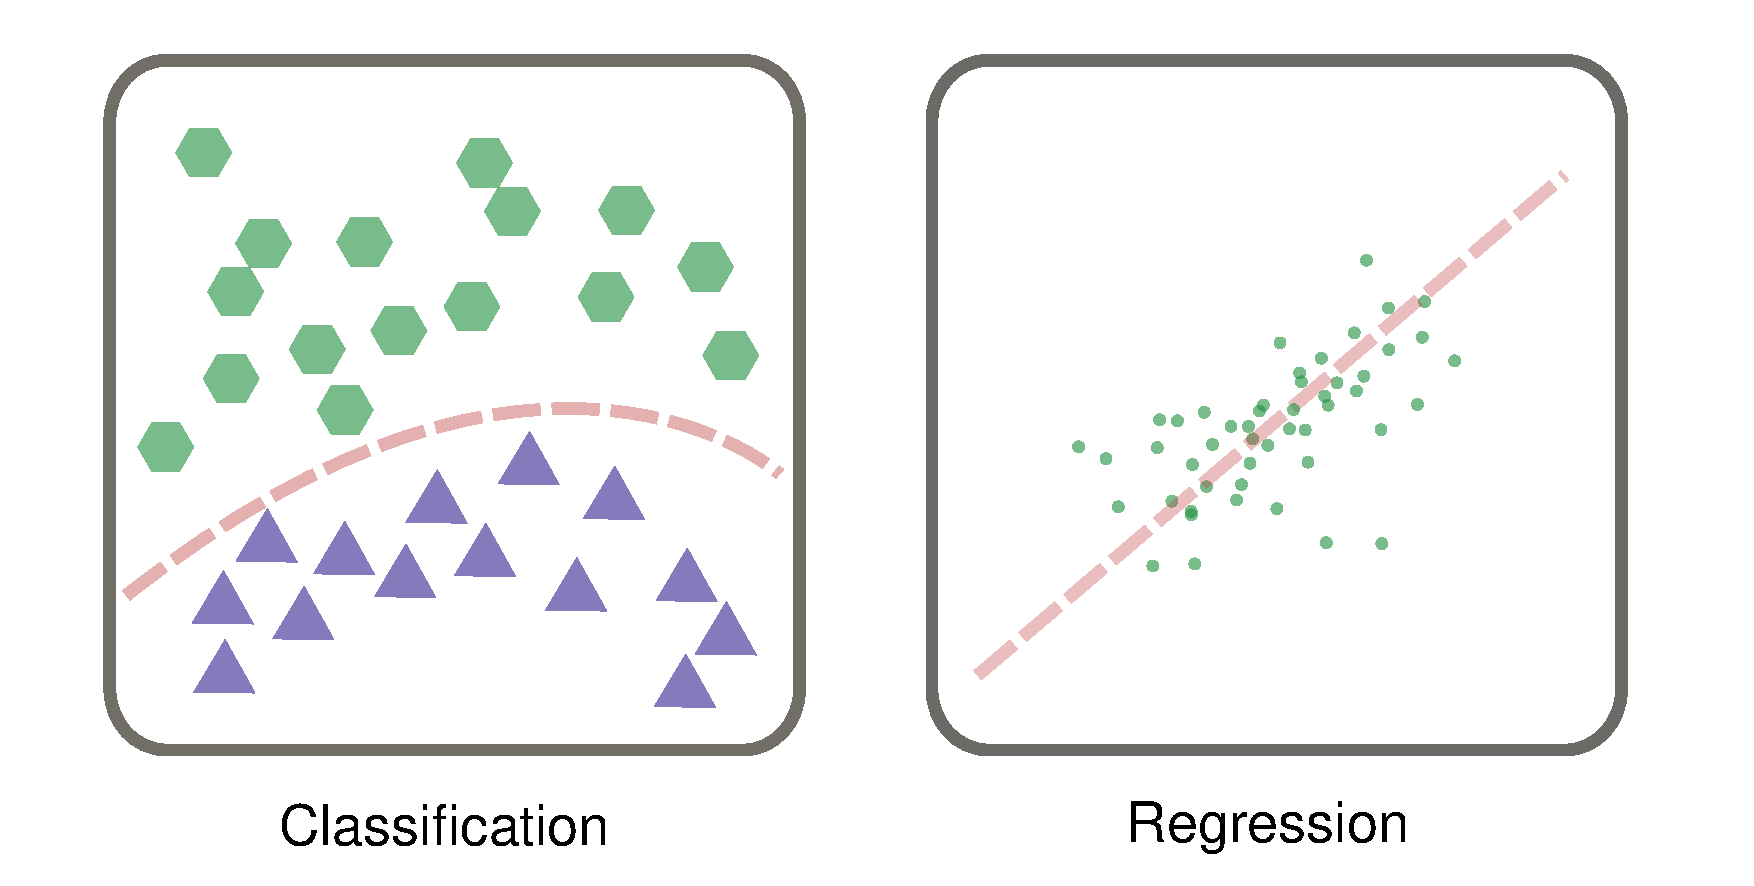
\includegraphics[width=13cm]{images/classification_and_regression.pdf}
  \end{center}
\end{frame}

\begin{frame}
  \frametitle{Classification types}
  \begin{center}
    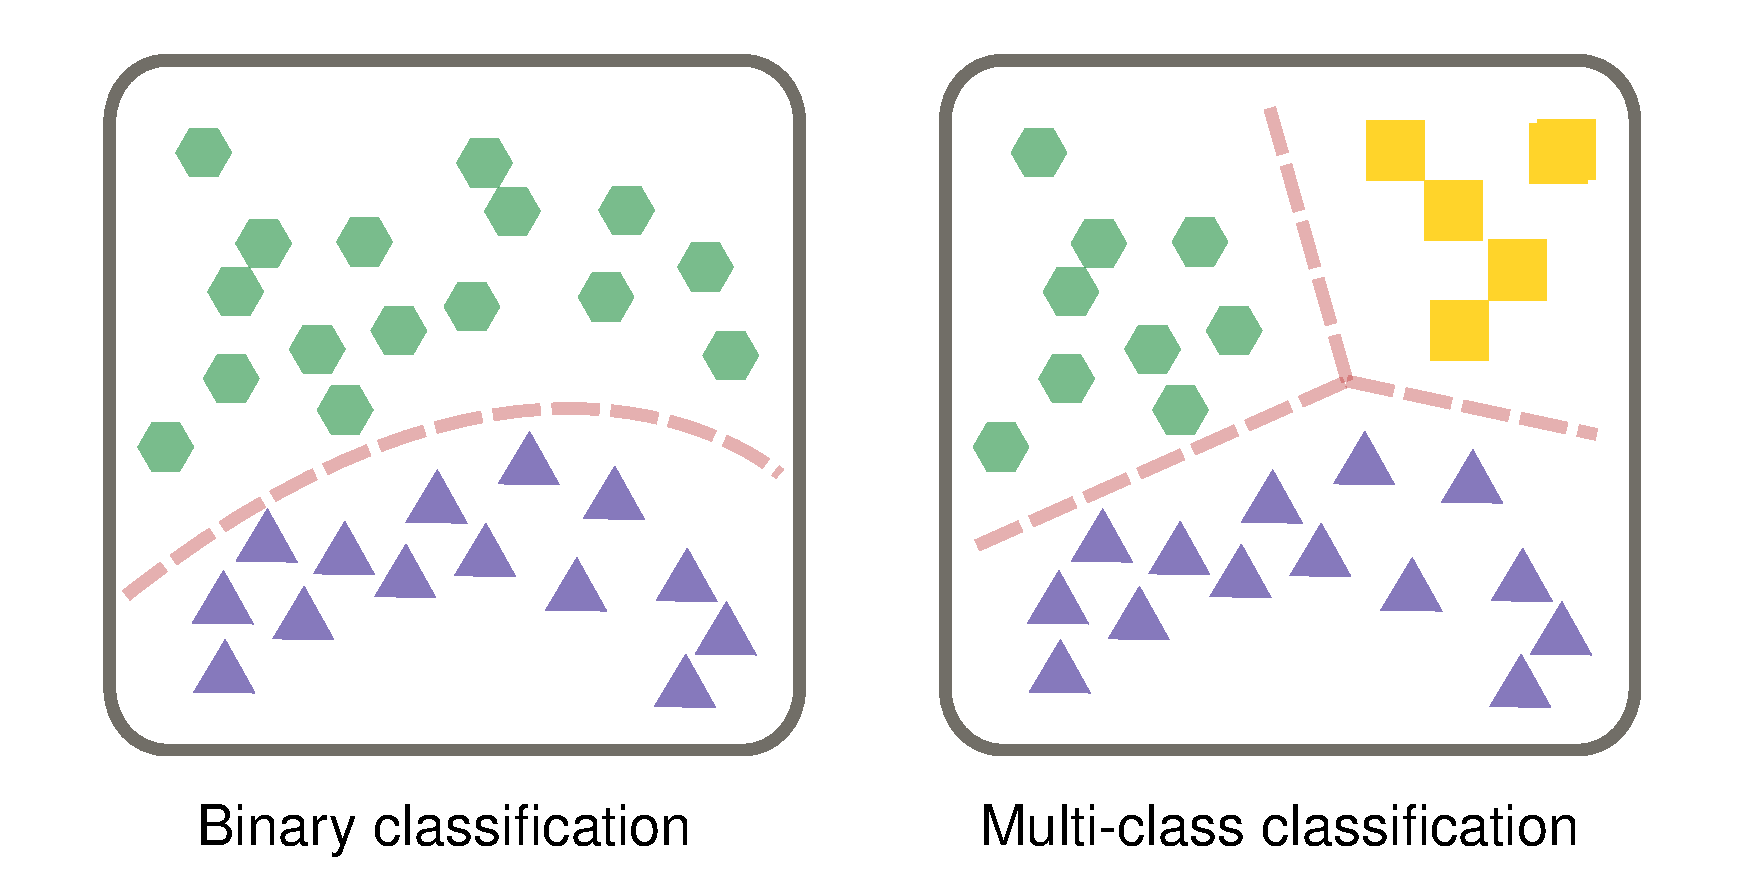
\includegraphics[width=13cm]{images/binary_vs_multi-class_classification.pdf}
  \end{center}  
\end{frame}

\begin{frame}
  \frametitle{Think-Pair-Share}
  \begin{block}{}
    \begin{center}
      Where in your research or your daily life have you\\
      experienced supervised machine learning?
    \end{center}    
  \end{block}
\end{frame}

%%%%%%%%%%%%%%%%%%%%%%
\section{Foundations and terms}
%%%%%%%%%%%%%%%%%%%%%%

\begin{frame}{}
   \tableofcontents[currentsection]
\end{frame}

\begin{frame}
  \frametitle{Entities and their features}
  \begin{block}{}
    \begin{center}
      \begin{itemize}
      \item Entities (aka. samples or data points) are described by
        features (aka.  covariates or attributes).
      \item Feature can be
        \begin{itemize}
        \item categorical
          \begin{itemize}
          \item Nominal (e.g. eye color, gender)
          \item Ordinal (e.g. very bad, bad, good, very good)
          \end{itemize}
        \item numerical
          \begin{itemize}
          \item Discrete (e.g. gene length in nucleotide)
          \item Continous (e.g. body length)
          \end{itemize}
        \end{itemize}
      \end{itemize}
    \end{center}
  \end{block}    
\end{frame}

\begin{frame}
  \frametitle{Features}
  \begin{block}{}
    \begin{center}
      \textbf{Feature selection}: Choosing the most descriptive
      features.
    \end{center}  
  \end{block}

  \begin{block}{}
    \begin{center}
      \textbf{Feature encoding}: Translating categorial values into
      numerical values.
    \end{center}  
  \end{block}  

  \begin{block}{}
    \begin{center}
      \textbf{Feature scaling}: Normalize feature values (e.g. scale
      by minimal and maximum values)
    \end{center}  
  \end{block}  
  
\end{frame}

\begin{frame}
  \frametitle{How well does the model fit?}

  \begin{block}{}
    \begin{center}
      \textbf{Overfitting}: Good performance on the training data, poor
      generalization to other data.\\      
    \end{center}
  \end{block}
  \begin{block}{}
    \begin{center}
      \textbf{Underfitting}: Poor performance on the training data and
      poor generalization to other data\\
    \end{center}
  \end{block}
  
  \begin{block}{}
    \begin{center}
      \textbf{Regularization}: Different methods to prevent overfitting\\
    \end{center}
  \end{block}
  
\end{frame}

%% \begin{frame}
%%   \frametitle{Evaluation of classificaions}

%%   Evaluation of binary classification - Confusion matrix for binary classification
  
%%   \begin{itemize}
%%   \item Positive (P): Observation is positive (for example: is an apple)
%%   \item Negative (N): Observation is not positive (for example: is not an apple).
%%   \item True Positive (TP): Observation is positive, and is predicted to be positive.
%%   \item False Negative (FN): Observation is positive, but is predicted negative.
%%   \item True Negative (TN): Observation is negative, and is predicted to be negative.
%%   \item False Positive (FP): Observation is negative, but is predicted positive.

%%   \item Accuracy
%%     ACC = (TP + TN) / (P + N)

%%   \item Recall sensitivity,  true positive rate
%%     TPR = TP / P

%%   \item Precision /  positive predictive value
%%     PPV = TP / (TP + FP)

%%   \item F1 (aka F-measure, F-score) - harmonic mean of precision and recall

%%     F1 = 2 * (1 / (1/recall) + (1/recall))
%%   \end{itemize}
  
%% \end{frame}


\begin{frame}
  \frametitle{Overview of different methods}
  \begin{block}{}
    \begin{center}
      \begin{itemize}
      \item Nearest Neighbor
      \item Naive Bayes
      \item Linear regression
      \item Logistic regression
      \item Decision Trees
      \item Artificial neural network (multilayer perceptron)
      \item Genetic Programming
      \end{itemize}
    \end{center}    
  \end{block}
\end{frame}

%%%%%%%%%%%%%%%%%%%%%%%%%%%%%%%%%%%%%%%%%%%%%%
\section{Selected supervised learning methods}
%%%%%%%%%%%%%%%%%%%%%%%%%%%%%%%%%%%%%%%%%%%%%%

\begin{frame}{}
   \tableofcontents[currentsection]
\end{frame}

%-------------------------------
\subsection{k-Nearest Neighbors}
%-------------------------------

\begin{frame}
  \frametitle{k-Nearest Neighbors}
  \begin{block}{}
    \begin{center}
      \begin{itemize}
      \item For classification and regression
      \item Simplest case of supervised machine learning
      \item Can be easily applied to multi-class classification
      \end{itemize}
    \end{center}
  \end{block}    
\end{frame}

\begin{frame}
  \frametitle{k-Nearest Neighbors}
  \begin{center}
    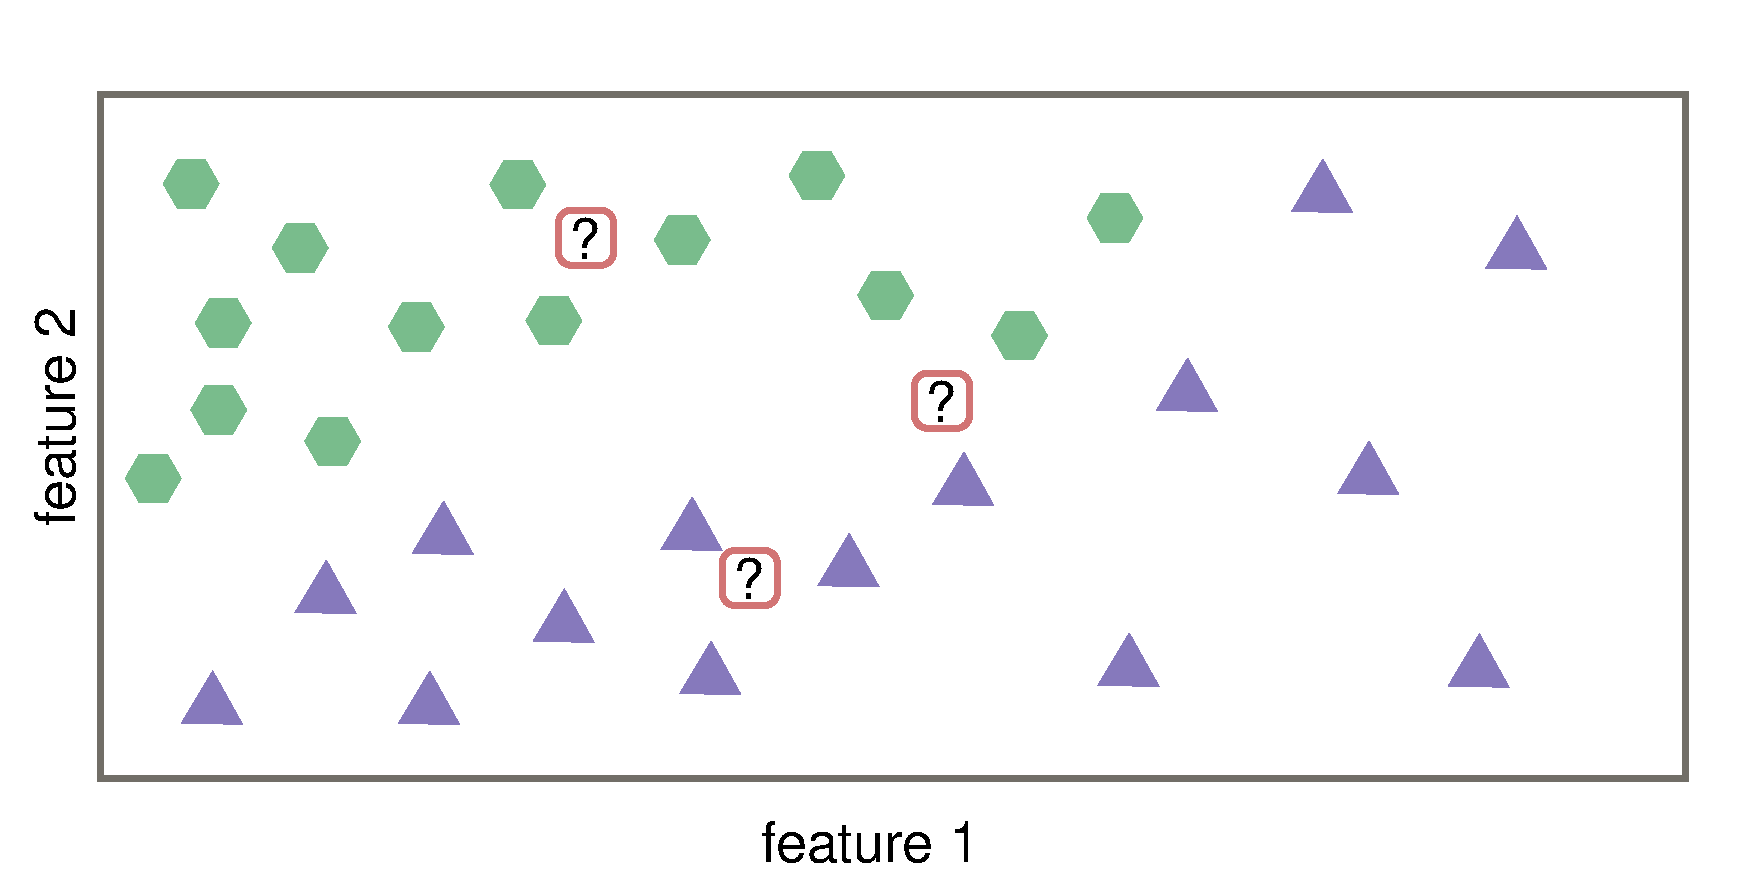
\includegraphics[width=13.0cm]{images/k_nearest_neighbour_classification_only_training_data.pdf}
  \end{center}
\end{frame}

\begin{frame}
  \frametitle{k-Nearest Neighbors}
  \begin{center}
    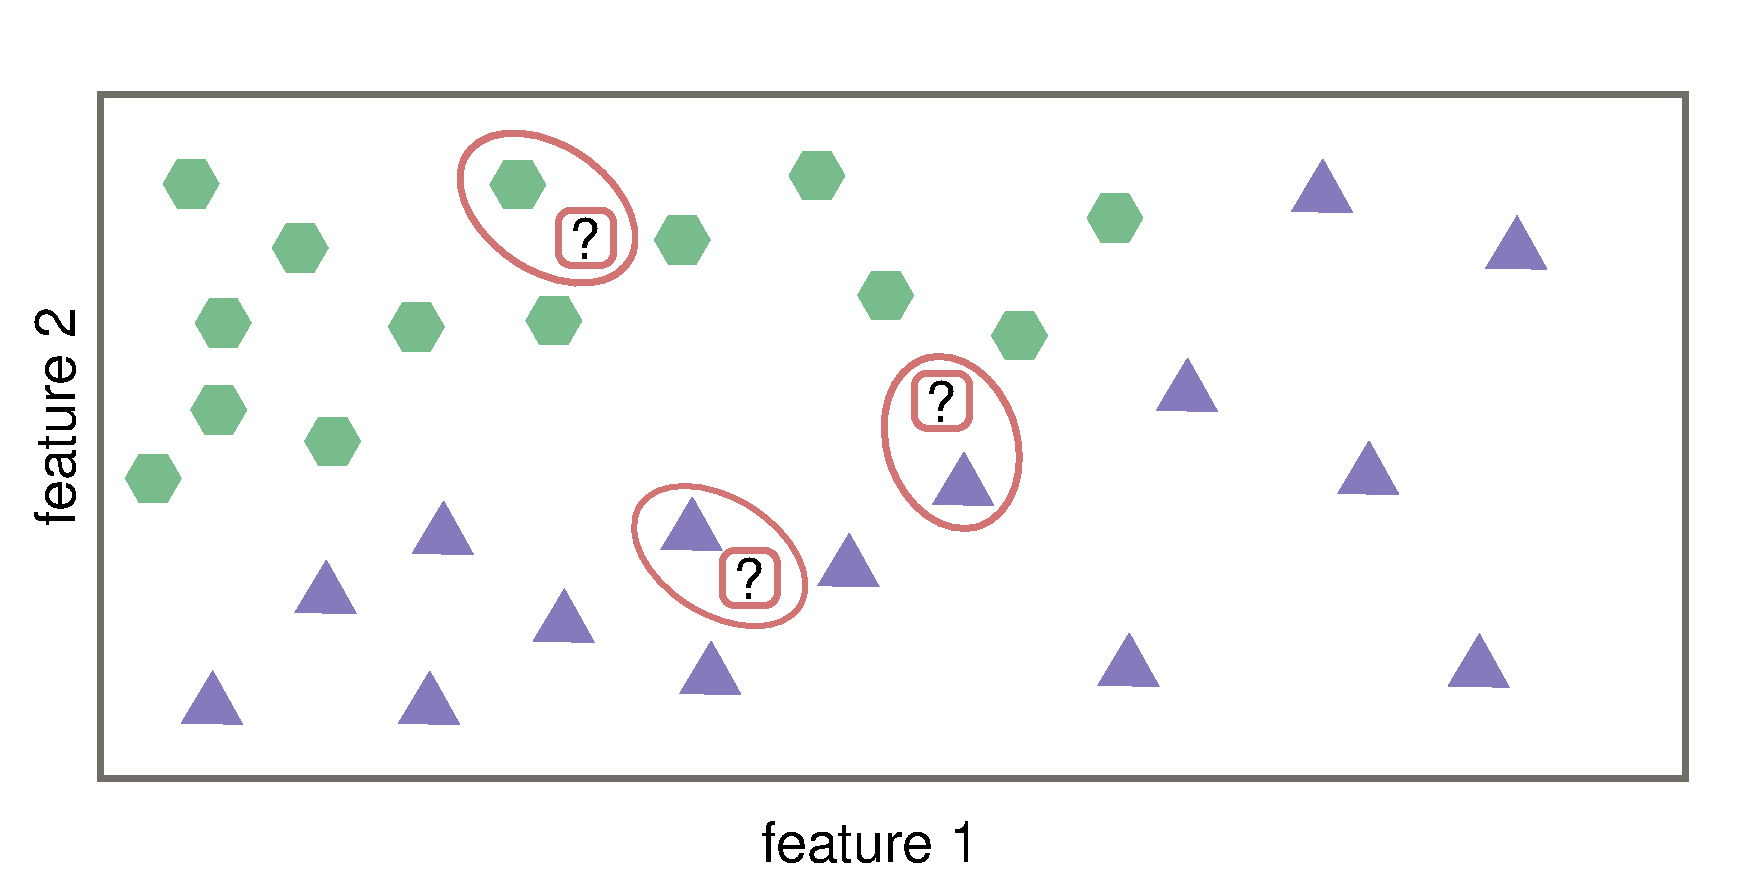
\includegraphics[width=13.0cm]{images/k_nearest_neighbour_classification_k_1.pdf}
  \end{center}
\end{frame}

\begin{frame}
  \frametitle{k-Nearest Neighbors}
  \begin{center}
    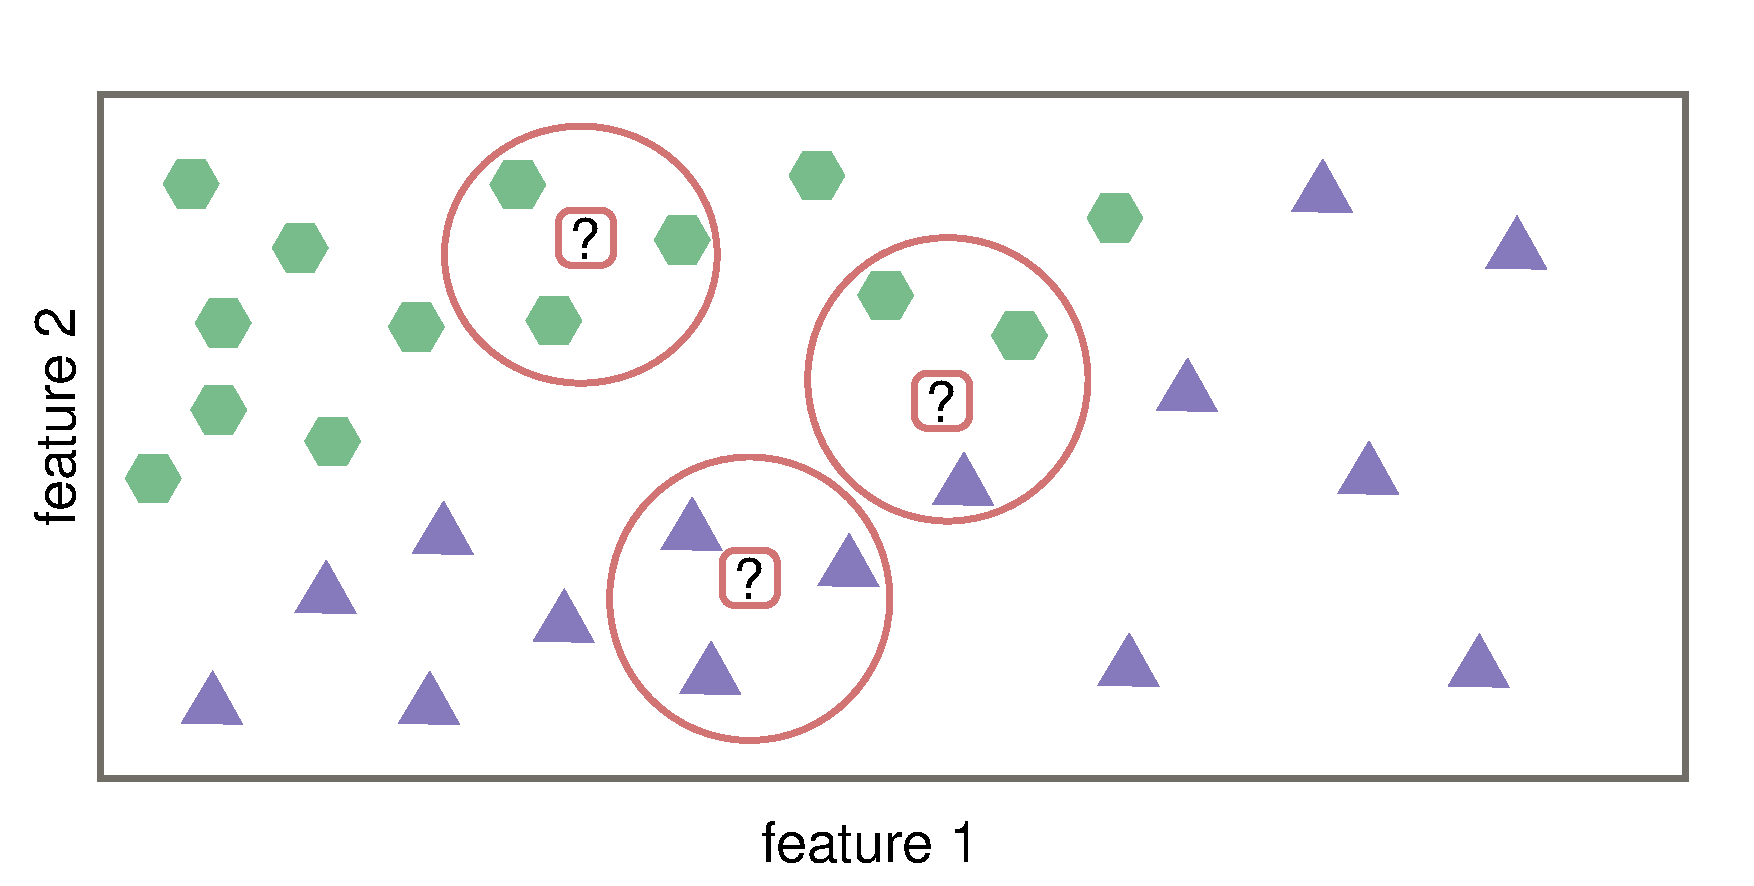
\includegraphics[width=13.0cm]{images/k_nearest_neighbour_classification_k_3.pdf}
  \end{center}
\end{frame}

\begin{frame}
  \frametitle{k-Nearest Neighbors}
  \begin{center}
    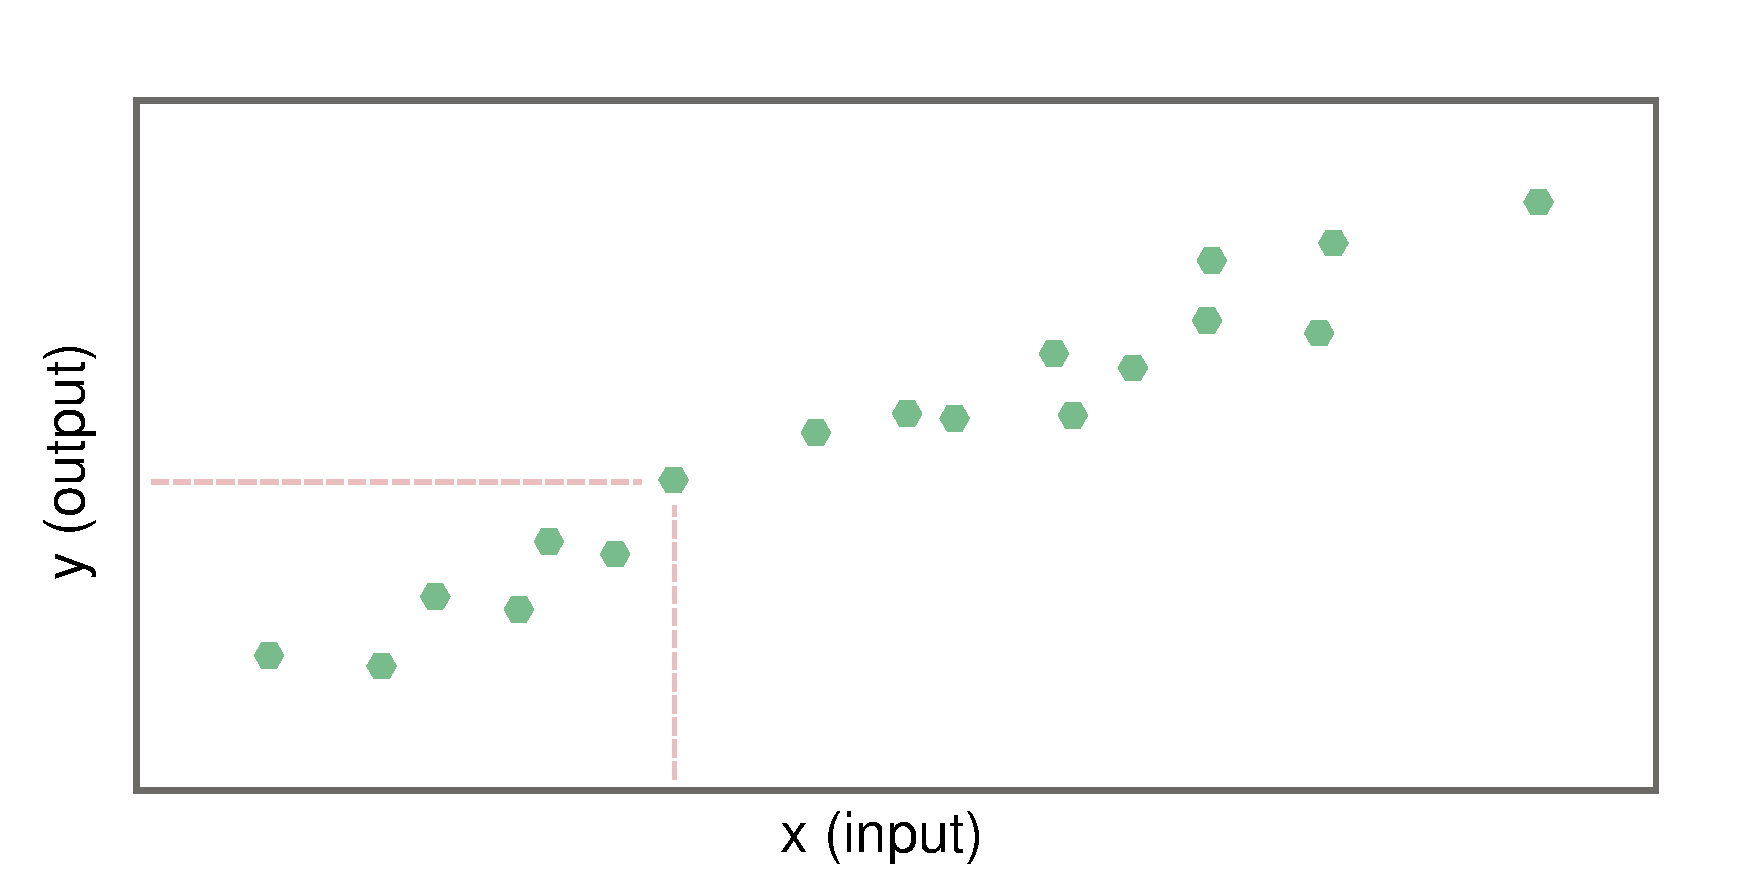
\includegraphics[width=13.0cm]{images/k_nearest_neighbour_regression_only_training_data.pdf}
  \end{center}
\end{frame}

\begin{frame}
  \frametitle{k-Nearest Neighbors}
  \begin{center}
    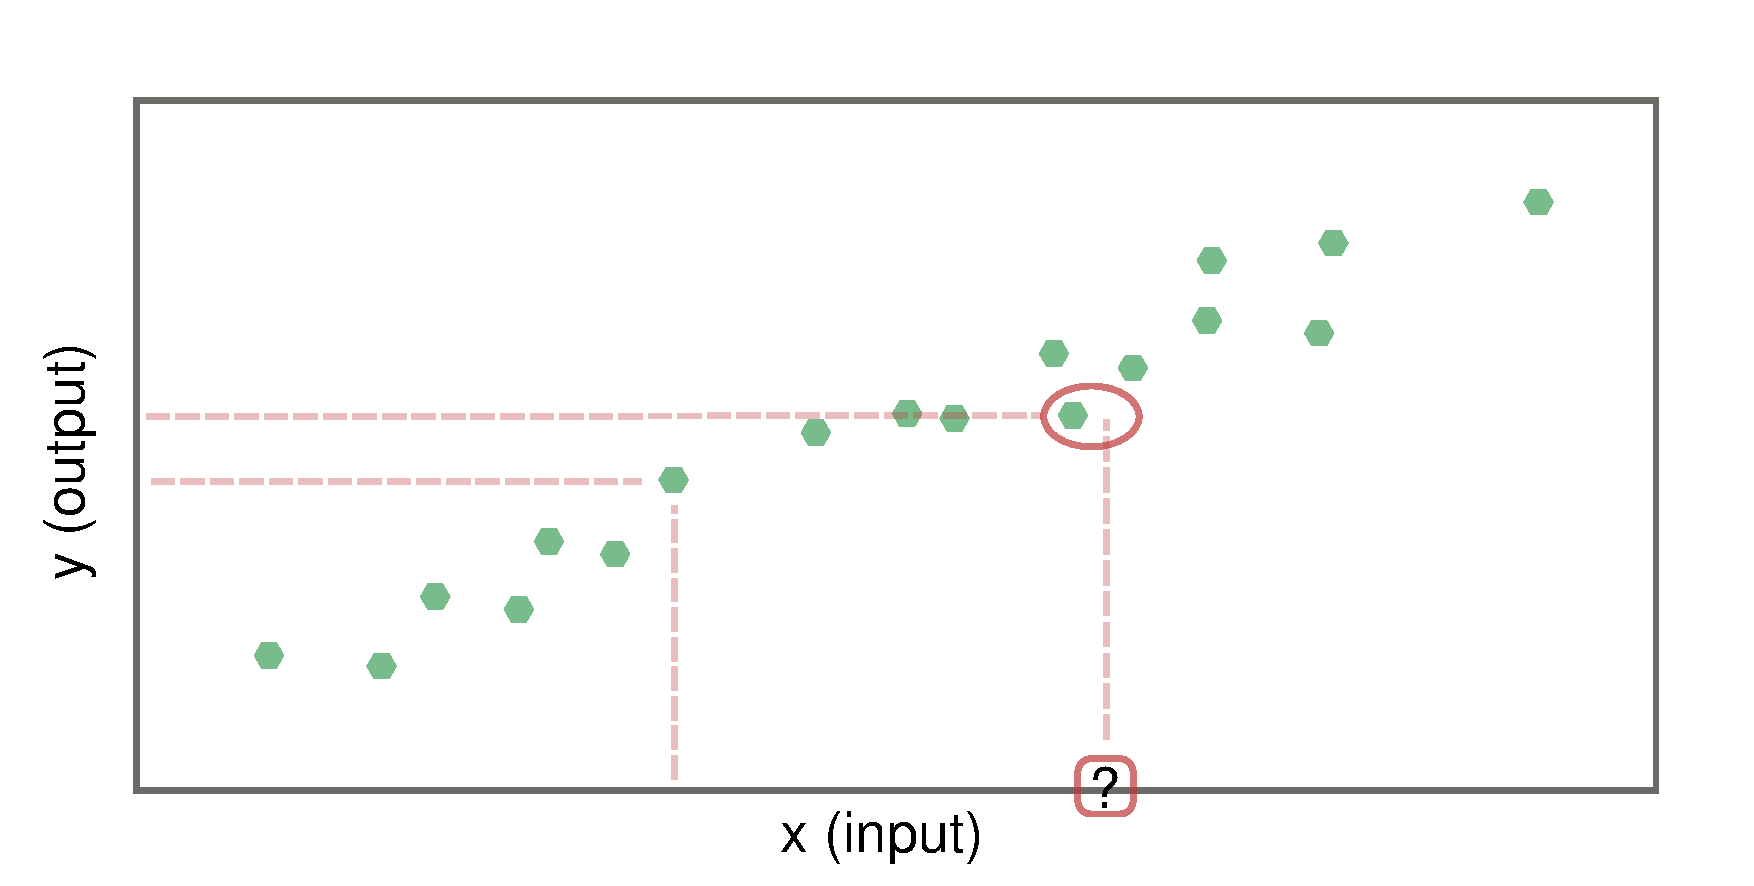
\includegraphics[width=13.0cm]{images/k_nearest_neighbour_regression_k_1.pdf}    
  \end{center}
\end{frame}

\begin{frame}
  \frametitle{k-Nearest Neighbors}
  \begin{center}
    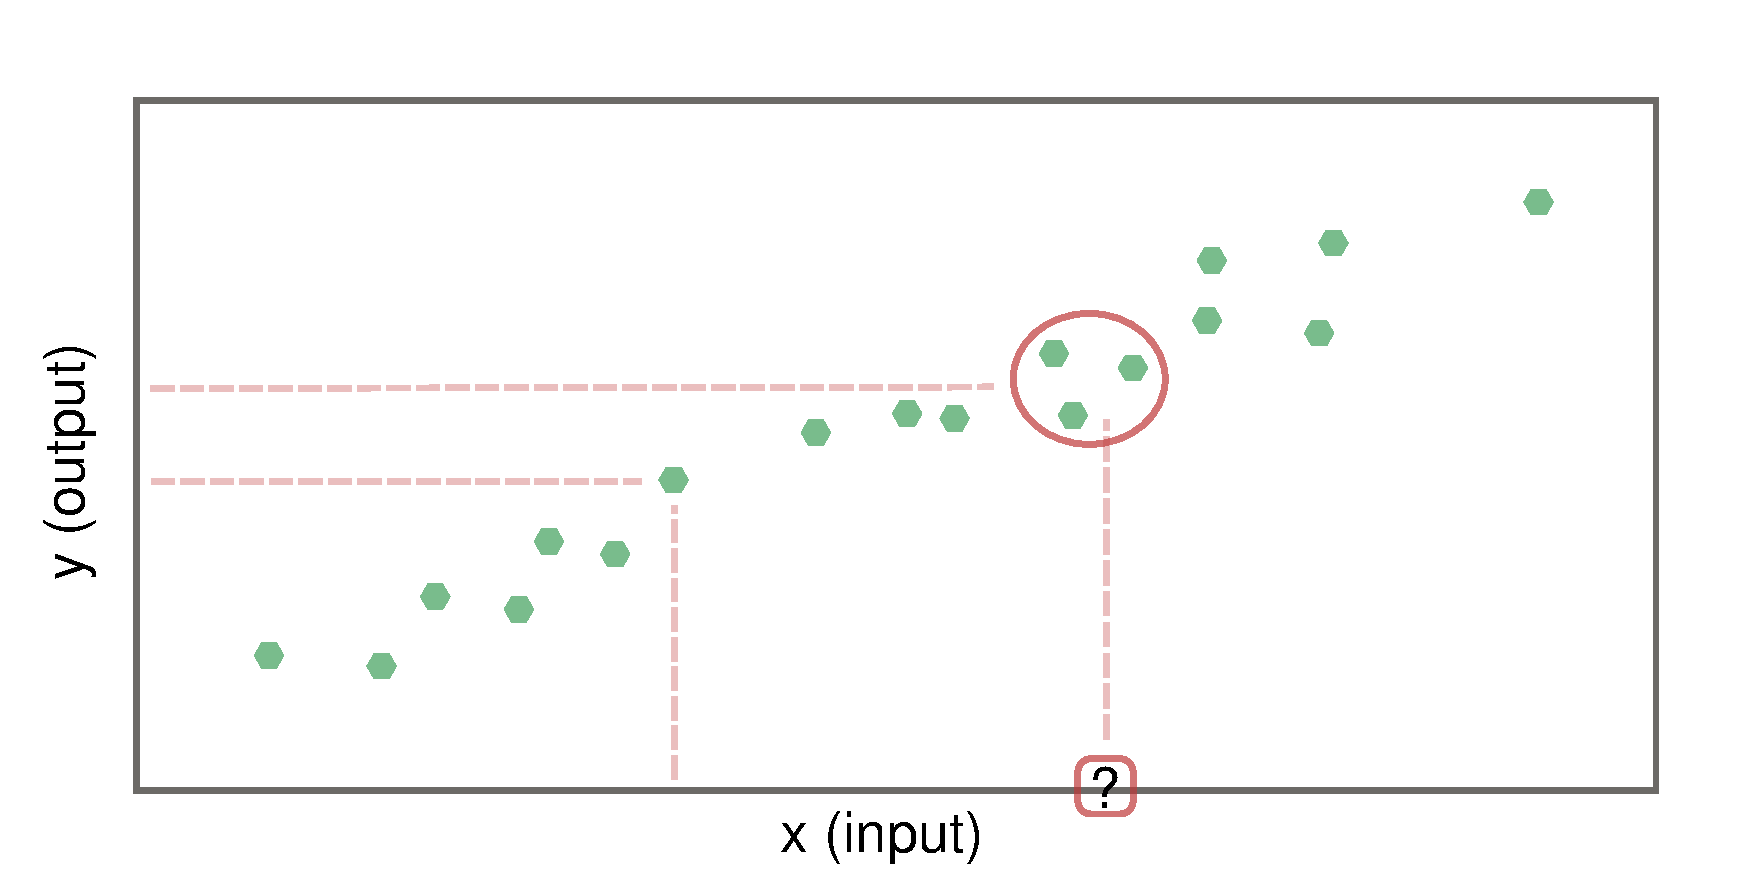
\includegraphics[width=13.0cm]{images/k_nearest_neighbour_regression_k_3.pdf}
  \end{center}
\end{frame}


%-------------------------
\subsection{Linear models}
%-------------------------

\begin{frame}
  \frametitle{Linear models}
  \begin{block}{}
    \begin{center}
      $\hat{y} = w_{1}x_{1} + w_{2}x_{2} + w_{3}x_{3} + ... + w_{n}x_{n} + b$\\
      \ \\
      with $n$ as the  number of features\\
      $w$ are the different weights/coefficients\\
      $b$ the intercept\\
    \end{center}
  \end{block}  
\end{frame}

\begin{frame}
  \frametitle{Different ways to estimate the parameters}
  \begin{block}{}
    \begin{center}
      \begin{itemize}
      \item Ordinary Least Squares
        \begin{itemize}
        \item no parameters - easy to use but no possibility to adapt
        \end{itemize}
      \item Ridge
        \begin{itemize}
        \item coefficients should be close to zero
        \item more resistant against overfitting
        \end{itemize}    
      \item Least Absolute Shrinkage and Selection Operator (LASSO)
      \end{itemize}
    \end{center}
  \end{block}
\end{frame}

\begin{frame}
  \frametitle{Ordinary least squares (OLS)}
  \begin{center}
    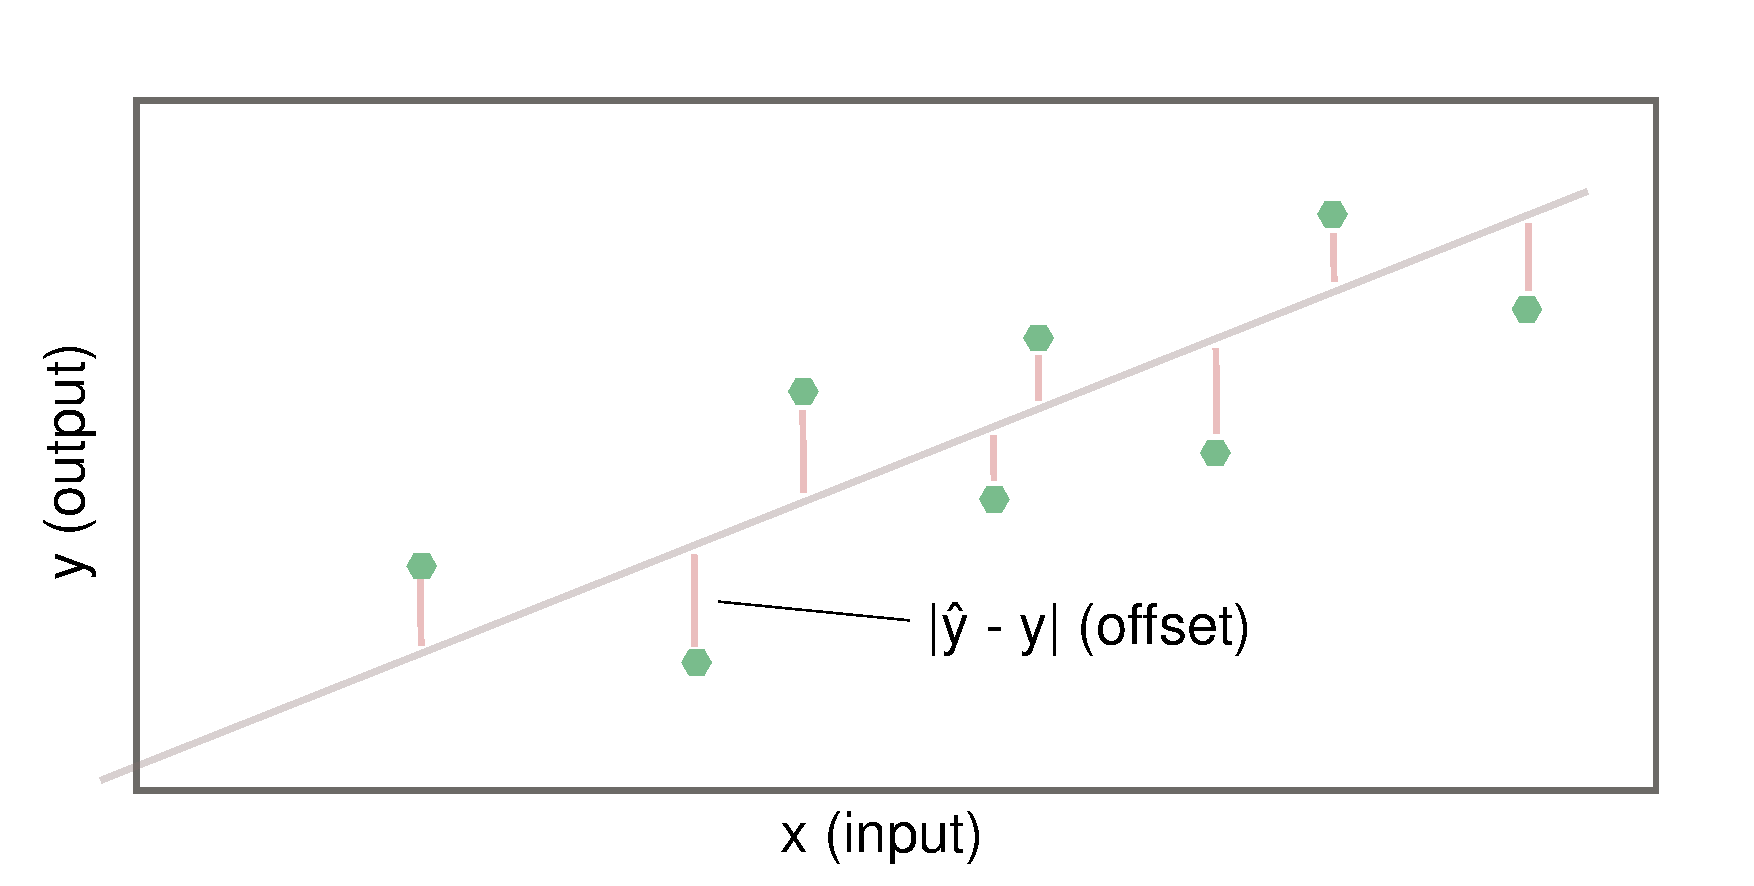
\includegraphics[width=13.0cm]{images/linear_model_ordinary_least_squares.pdf}
    Minimize the offset between $\hat{y}$ and $y$ the\\
    mean squared error (MSE) or sum of squared errors (SSE).
  \end{center}
\end{frame}


\begin{frame}
  \frametitle{}
  \begin{block}{}
    \begin{center}
      Once the parameters ($b$ and the weights $w$) of\\
      \ \\
      $\hat{y} = w_{1}x_{1} + w_{2}x_{2} + w_{3}x_{3} + ... + w_{n}x_{n} + b$\\
      \ \\
      are estimated the prediction can be performed\\
      by putting the x values of the data points into the\\
      equation to predict the y value.
    \end{center}
  \end{block}
\end{frame}

%-----------------------------------------
\subsection{Support Vector Machine (SVMs)}
%-----------------------------------------

\begin{frame}
  \frametitle{SVM -- Separeting hyperplan}
  \begin{center}
    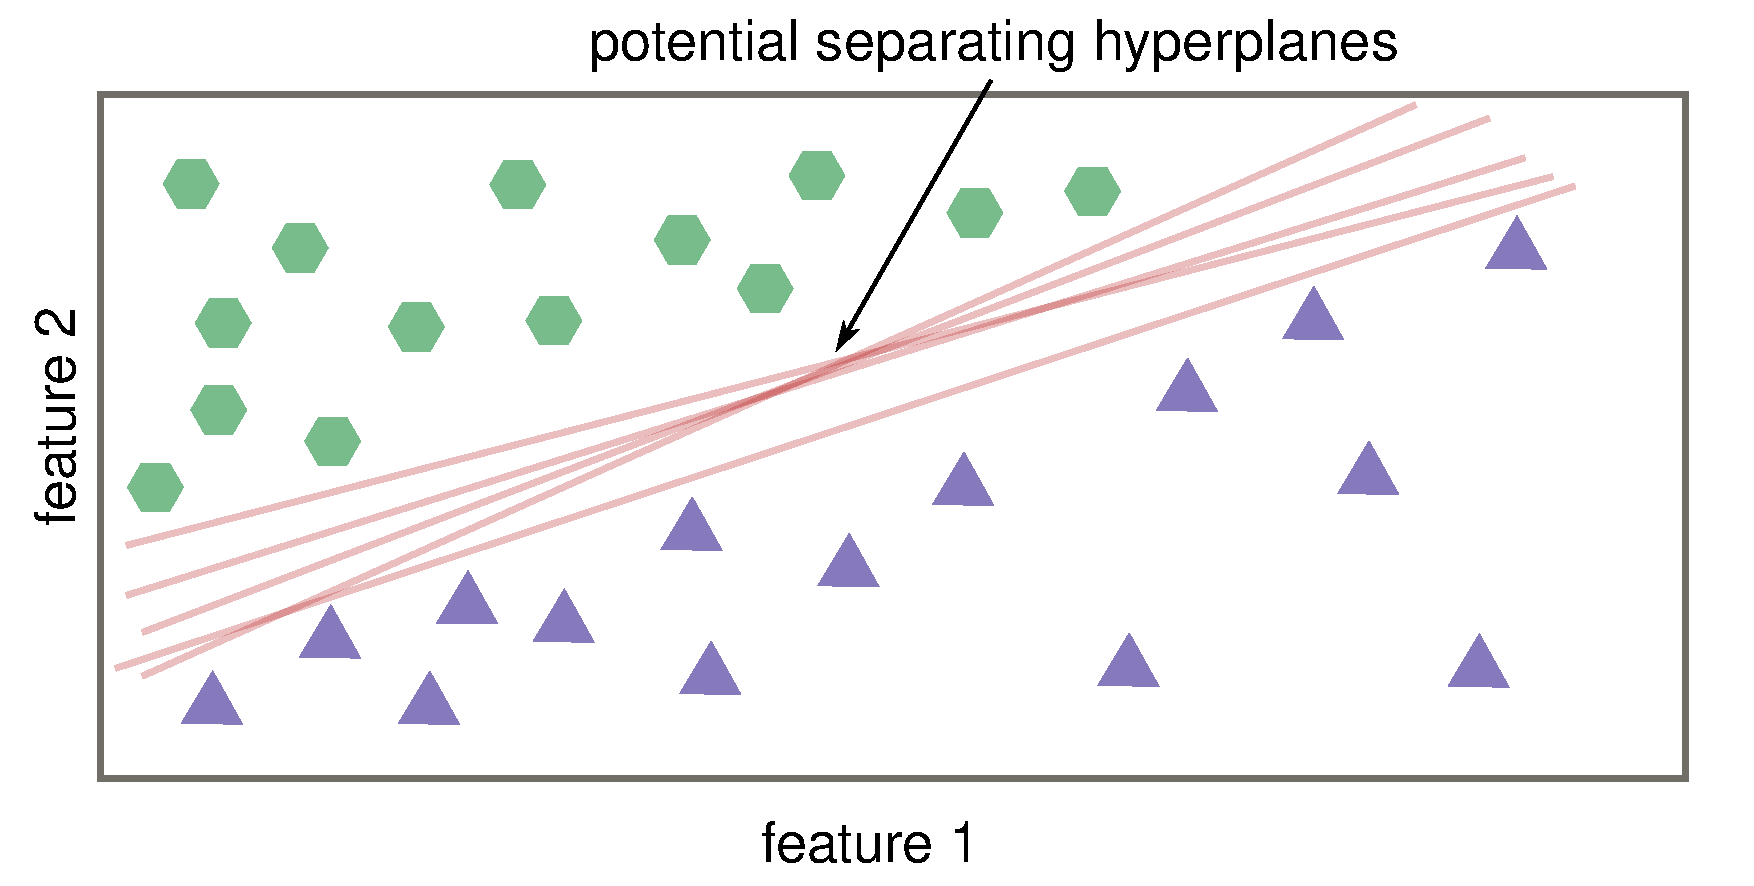
\includegraphics[width=13.0cm]{images/svm_potential_separating_hyperplanes.pdf}
  \end{center}
\end{frame}

\begin{frame}
  \frametitle{SVM -- Margin}
  \begin{center}
    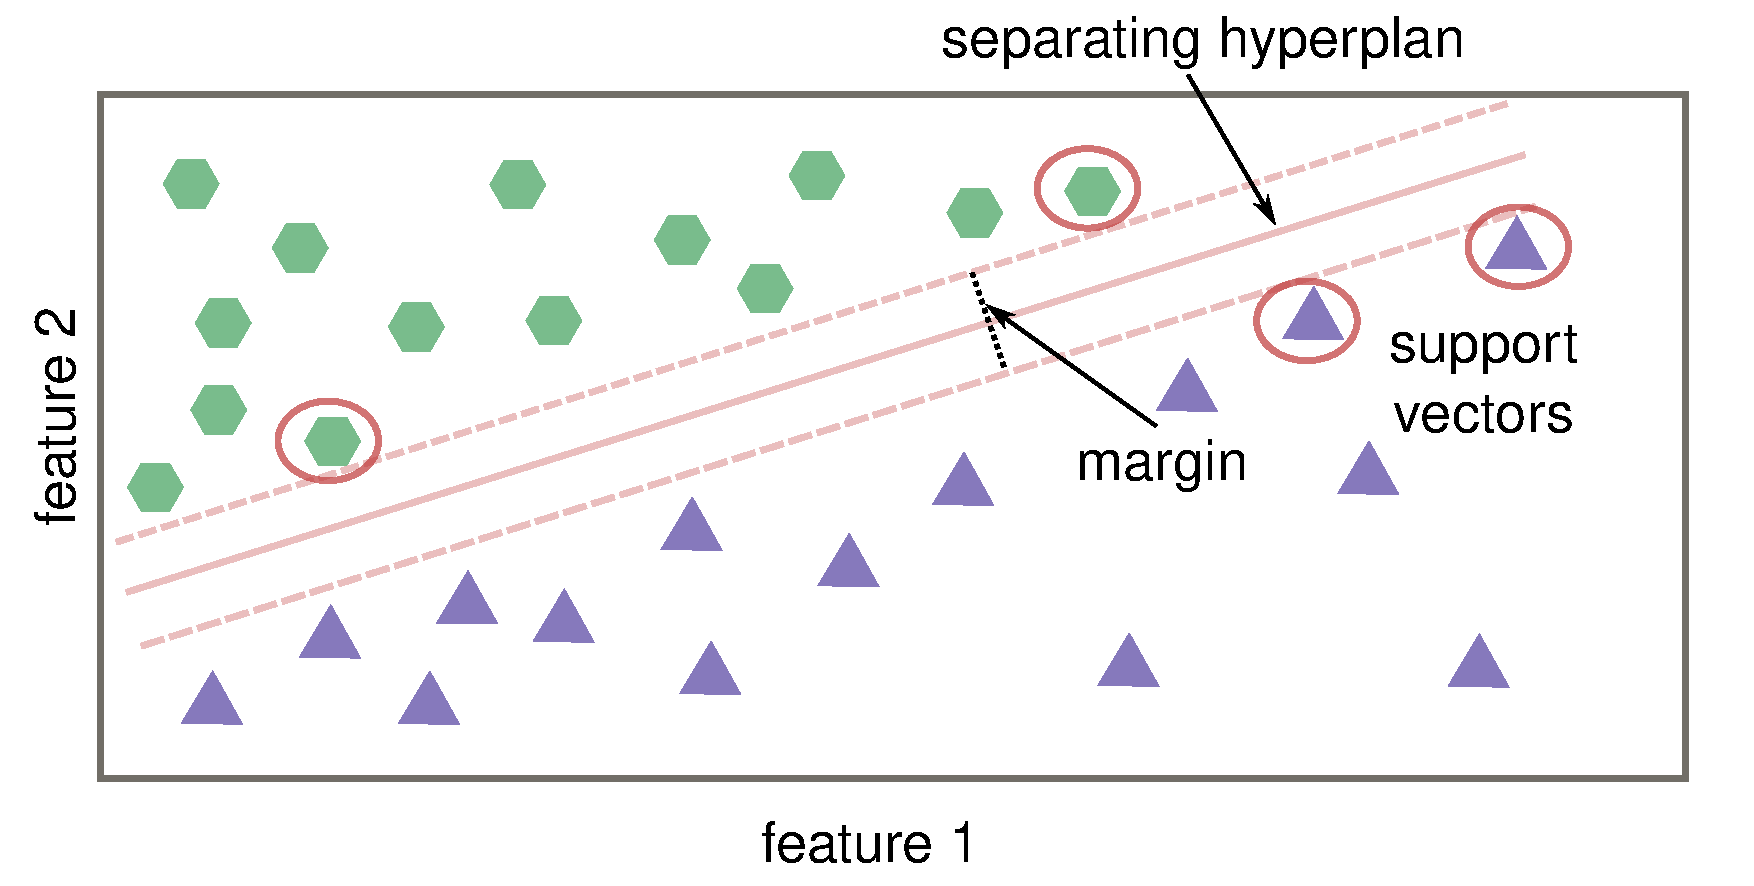
\includegraphics[width=13.0cm]{images/svm_with_margin.pdf}
  \end{center}
\end{frame}

\begin{frame}
  \frametitle{SVM -- Soft Margin}
  \begin{center}
    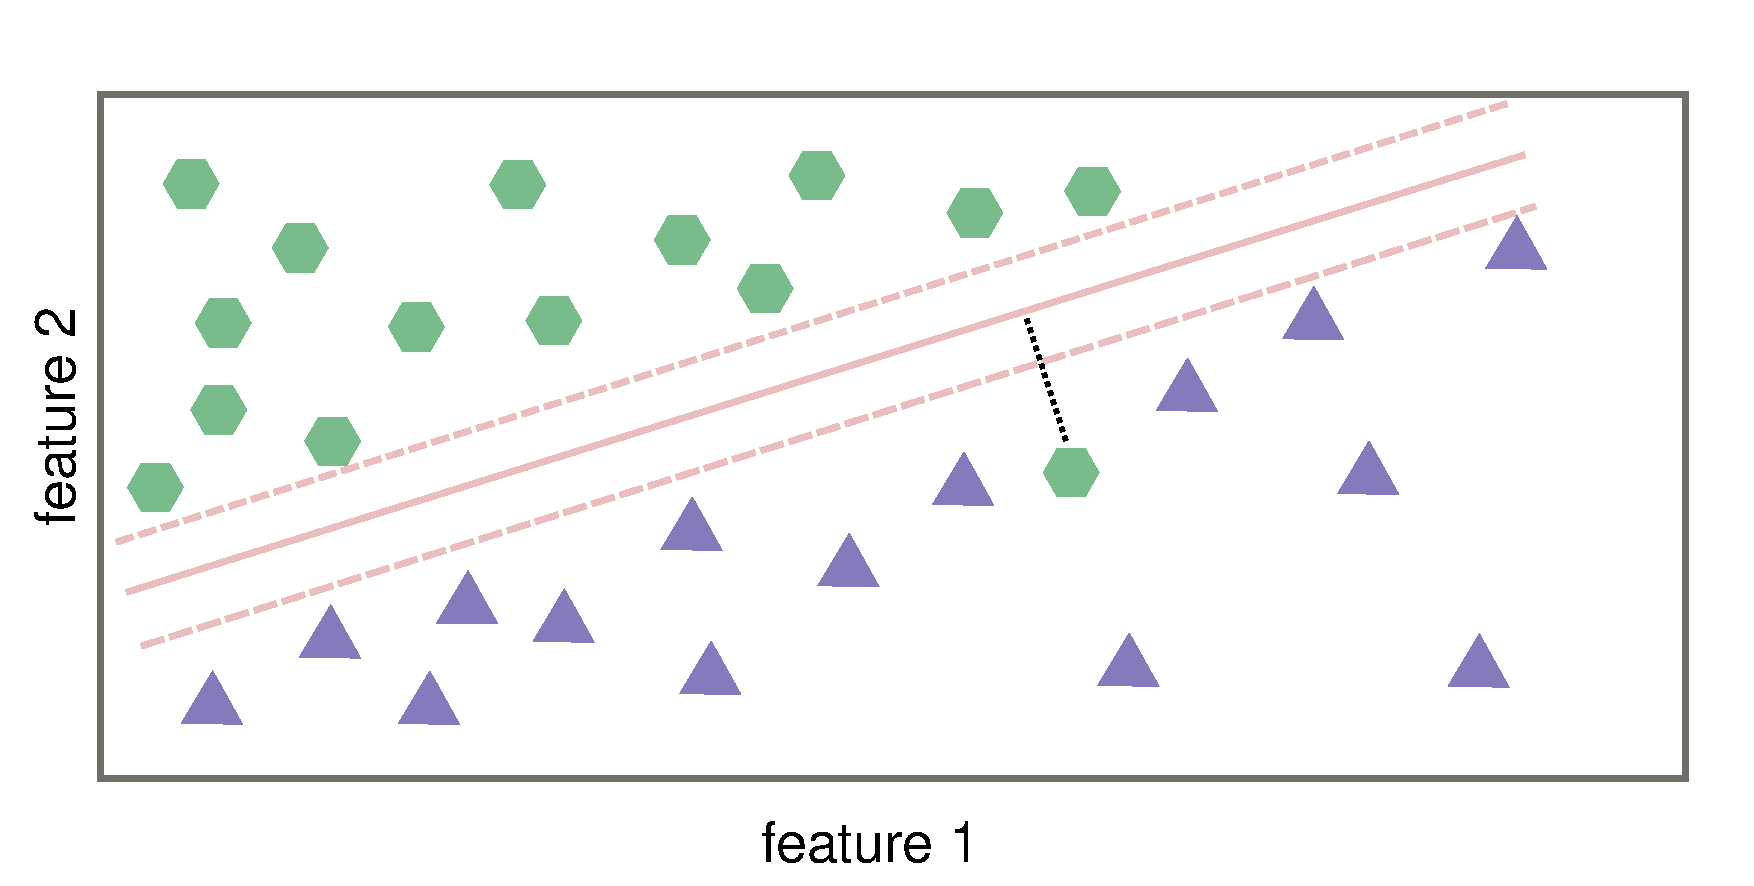
\includegraphics[width=13.0cm]{images/svm_with_soft_margin.pdf}
  \end{center}
\end{frame}

\begin{frame}
  \frametitle{SVM -- Kernel trick}
  \begin{center}
    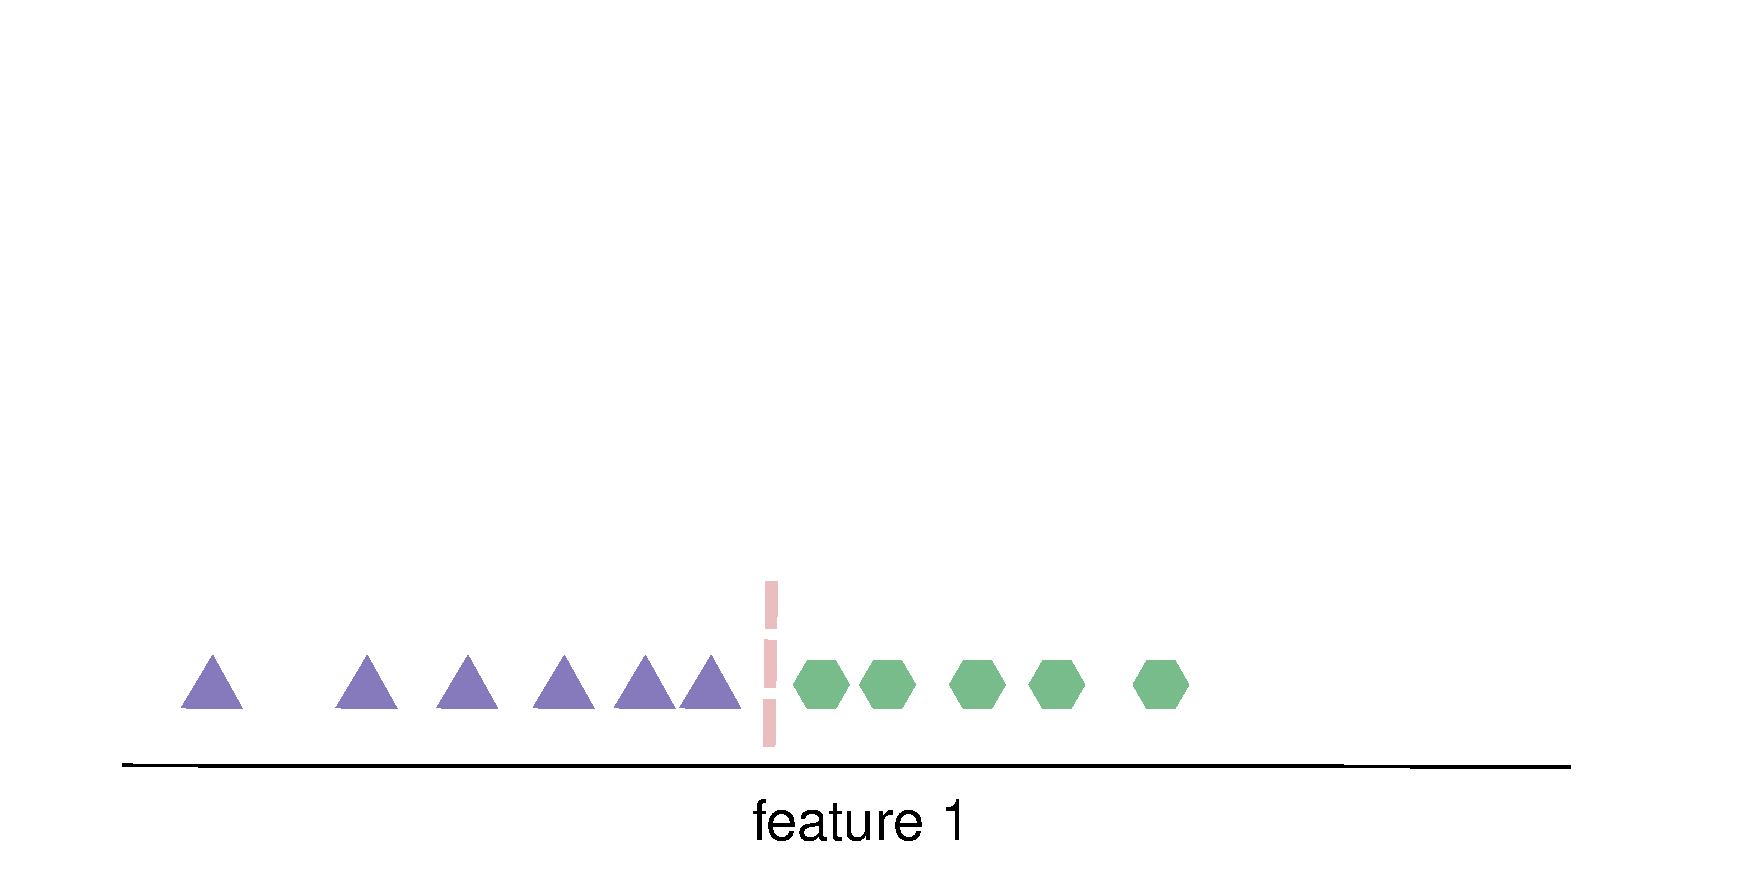
\includegraphics[width=13.0cm]{images/svm_kernel_trick_1.pdf}
  \end{center}
\end{frame}

\begin{frame}
  \frametitle{SVM -- Kernel trick}
  \begin{center}
    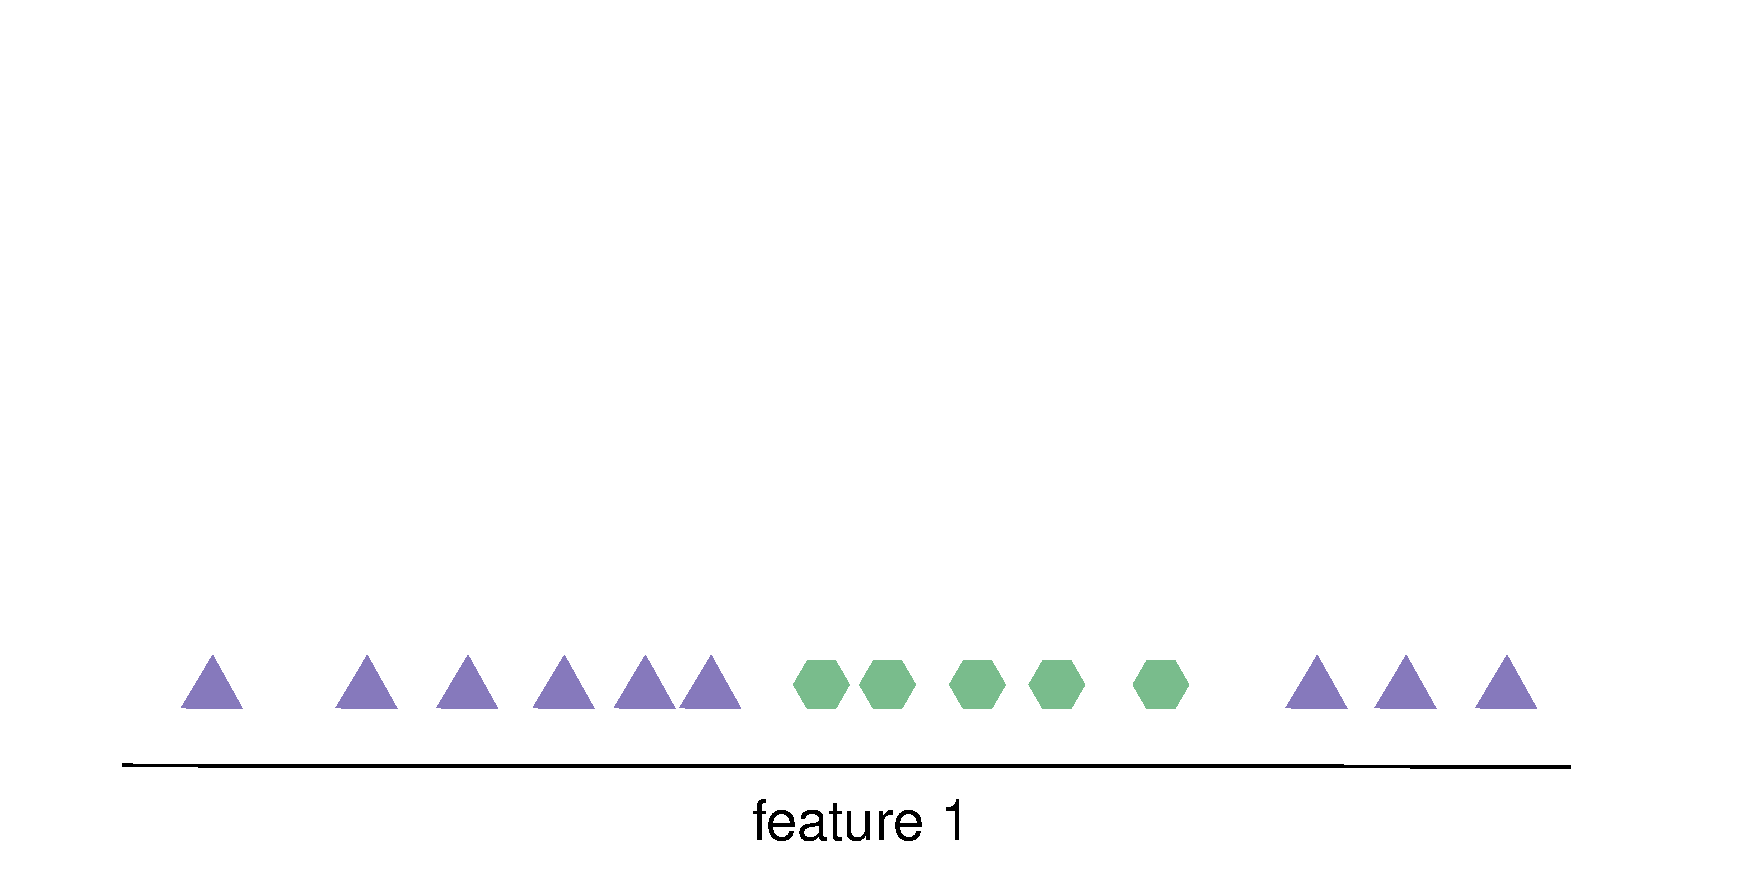
\includegraphics[width=13.0cm]{images/svm_kernel_trick_2.pdf}
  \end{center}
\end{frame}

\begin{frame}
  \frametitle{SVM -- Kernel trick}
  \begin{center}
    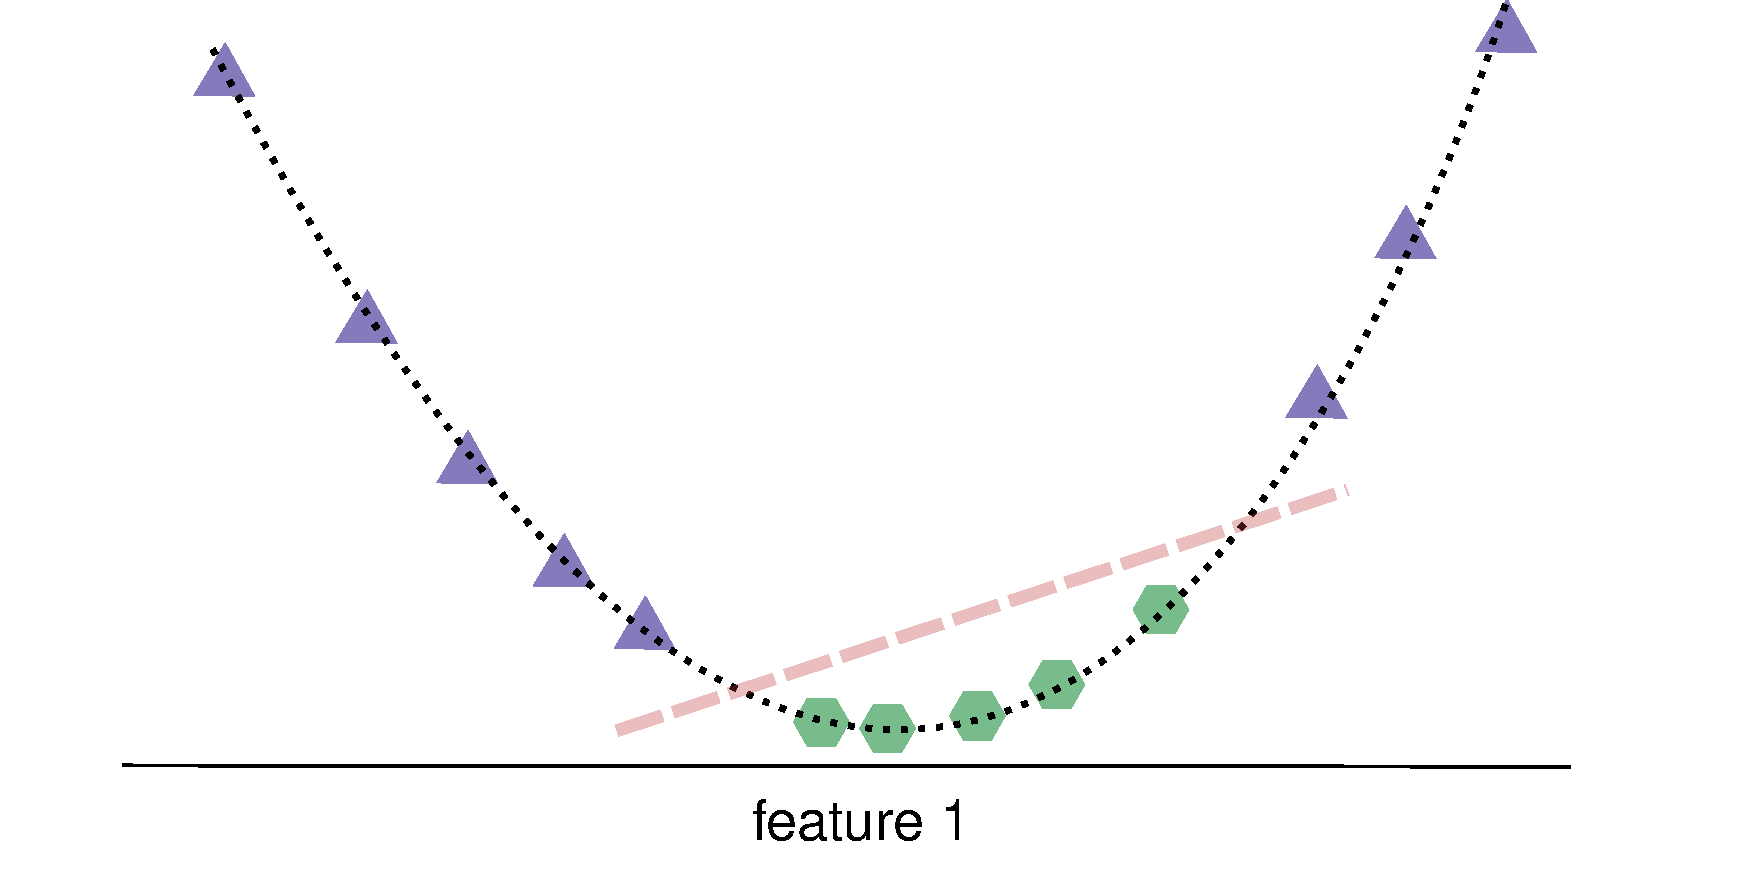
\includegraphics[width=13.0cm]{images/svm_kernel_trick_3.pdf}
  \end{center}
\end{frame}

%\section{Multiclass classification}

%% \begin{itemize}
%% \item Combining several SVMs e.g. train multiple one-versus-all classifiers
%% \end{itemize}
%% \end{frame}


%-------------------------
\subsection{Decision trees and Random forest}
%-------------------------

\begin{frame}
  \frametitle{Decision Trees}
  \begin{center}
    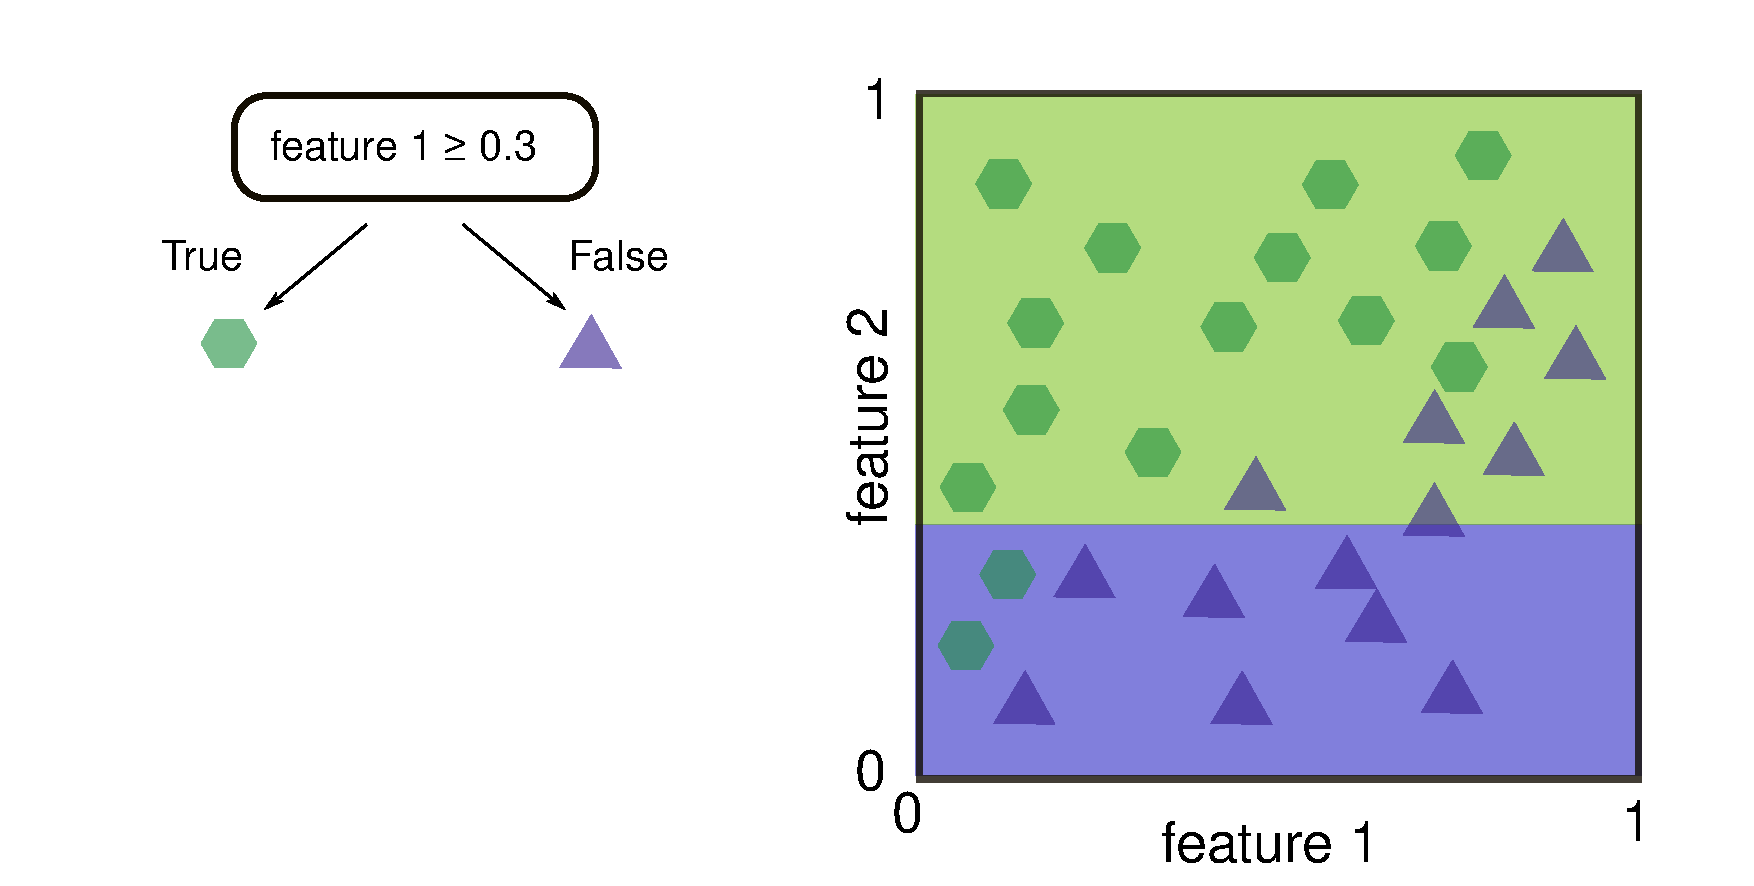
\includegraphics[width=13.0cm]{images/decision_tree_1.pdf}
  \end{center}  
\end{frame}

\begin{frame}
  \frametitle{Decision Trees}
  \begin{center}
    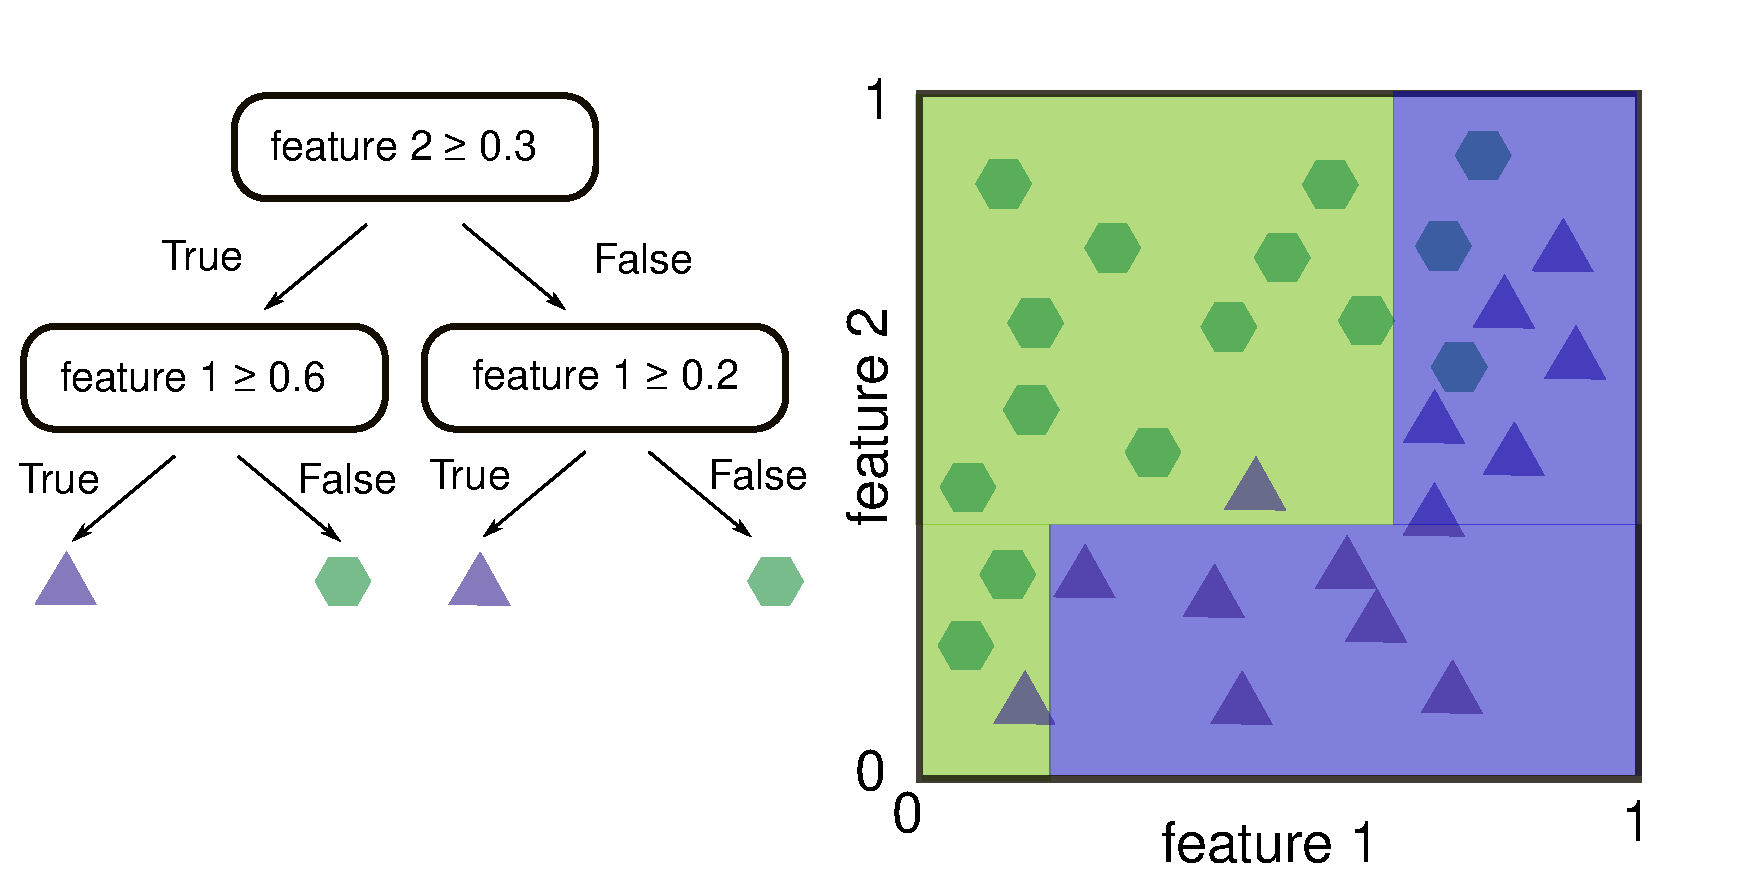
\includegraphics[width=13.0cm]{images/decision_tree_2.pdf}
  \end{center}  
\end{frame}

%% \begin{frame}
%%   Decision trees
%%   \begin{itemize}
%%   \item Concepts:
%%   \item node
%%   \item edge
%%   \item root
%%   \item leaf
%%   \item child
%%   \item parent
%%   \item A forest is a set of n ≥ 0 disjoint trees
%%   \item features: real-valued or categorial and also missing values
%%   \end{itemize}
%% \end{frame}

\begin{frame}
  \frametitle{Random forest}
  \begin{block}{}
    \begin{center}
      \begin{itemize}
      \item In the random forests approach, many different decision trees
        are grown by a randomized tree-building algorithm.
      \item The training set is sampled with replacement to produce a
        modified training set of equal size to the original but with some
        training items included more than once.
      \item In addition, when choosing the question at each node, only a
        small, random subset of the features is considered.
      \item Random decision trees from subsets of features or data point
      \end{itemize}
    \end{center}
  \end{block}
\end{frame}

%--------------------------------------
\subsection{Artificial Neural Networks}
%--------------------------------------

\begin{frame}
  \begin{block}{}
    \begin{center}
      \frametitle{Artificial Neural Networks}
      \begin{itemize}
      \item aka. Multilayer perceptrons or Feed-forward neural networks
      \item Inspired by natural Neural Networks
      \item For classification or regression
      \end{itemize}
    \end{center}  
  \end{block}  
\end{frame}


\begin{frame}
  \frametitle{Artificial Neural Networks}
  \begin{center}    
    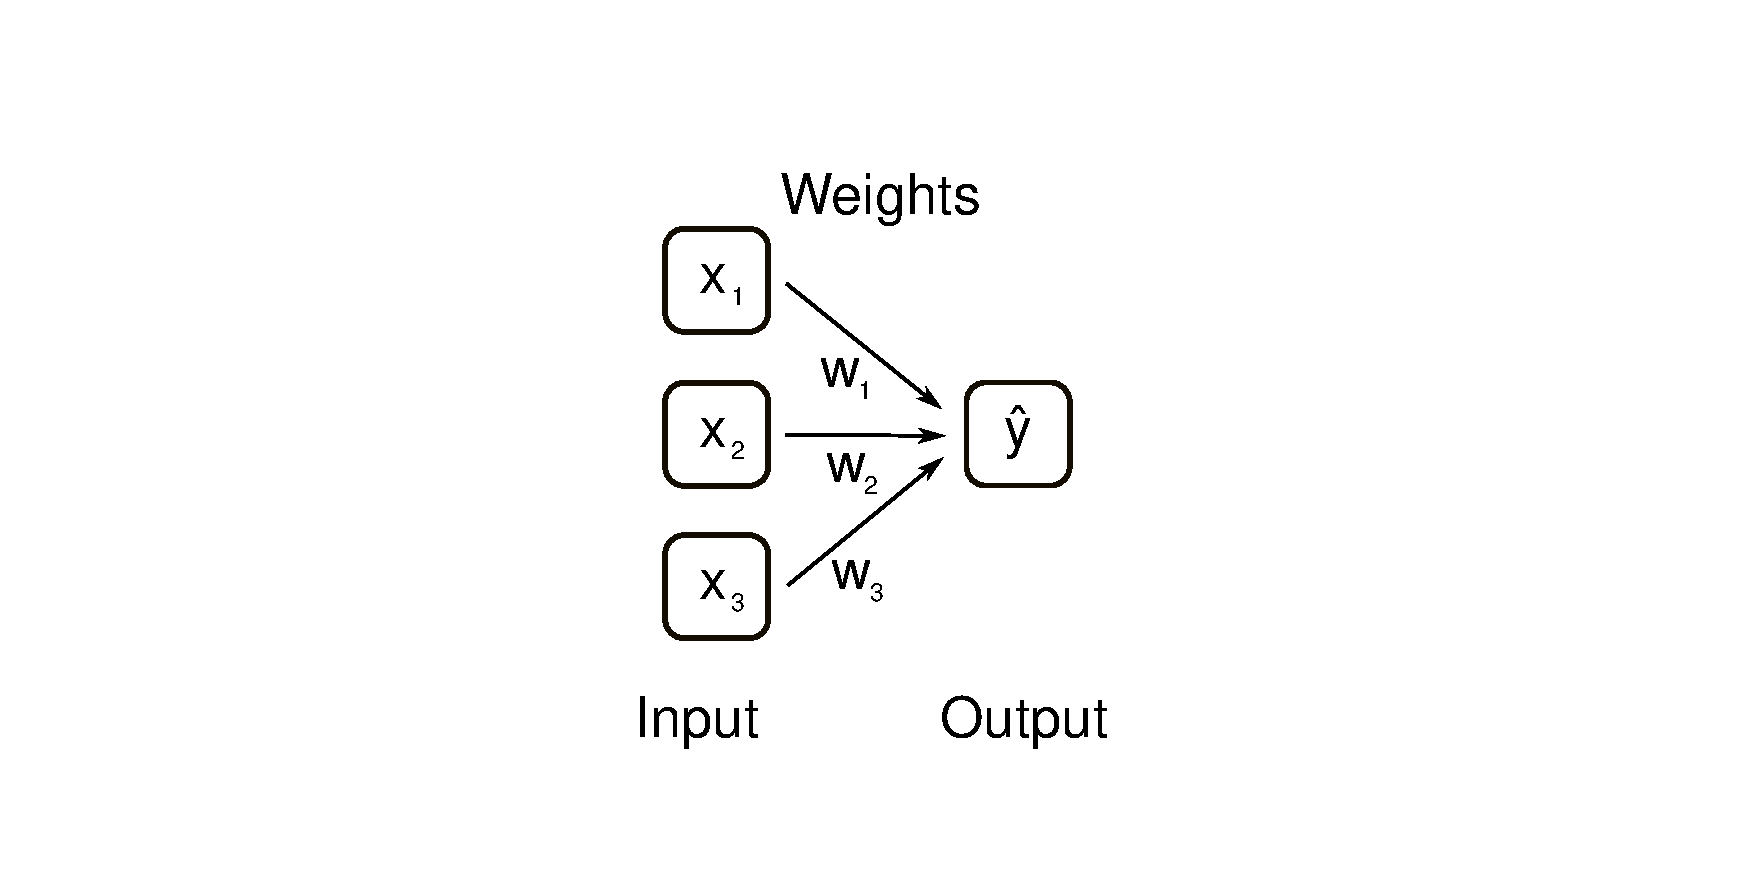
\includegraphics[width=13.0cm]{images/ANN_without_hidden_layer.pdf}
  \end{center}  
\end{frame}

\begin{frame}
  \frametitle{Artificial Neural Networks}
  \begin{center}
    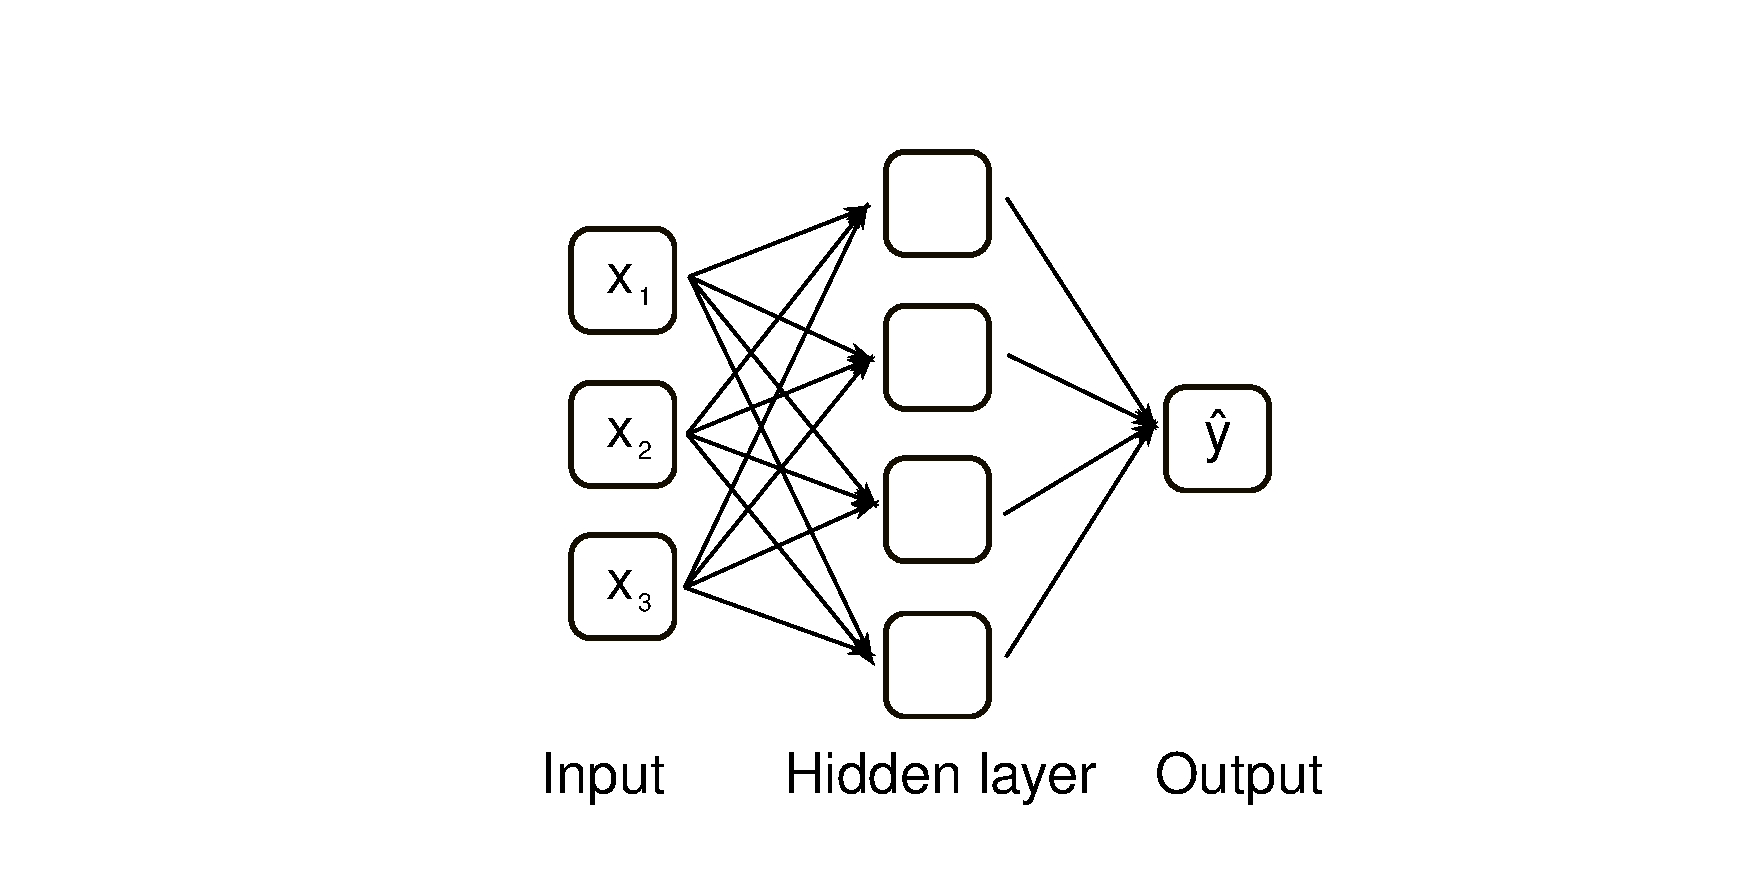
\includegraphics[width=13.0cm]{images/ANN_with_hidden_layer.pdf}
  \end{center}  
\end{frame}

\end{document}
